\documentclass[thesis.tex]{subfiles}

\begin{document}

Coupled-cluster theory is a powerful method for approximating solutions to the many-body Schr\"odinger equation.  Because of its effectiveness and economical scaling it has been a staple of many-body quantum mechanics for decades.  This chapter details various aspects of the coupled-cluster approach and presents ground-state results for multiple systems.  First, the CC wave operator and the corresponding effective Hamiltonian will be introduced and used to derive the CC equations.  Then, results from MBPT are used to illuminate the underlying many-body physics of the CC wave function.  After the mathematical foundations of coupled cluster theory are outlined, specific implementation details are discussed and demonstrated by focusing on two simple examples.  Finally, the nuclear many-body problem is formally introduced, along with a brief description of the nuclear interactions used in this work, and selected results are shown.

\section{Exponential Ansatz} \label{section:exponentialansatz}

Coupled cluster theory is based on expressing the $A$-particle correlated wave function $\corrket$ using the exponential ansatz \cite{COESTER1960477,CIZEK19664256},
\begin{equation} \label{eq:cc_ansatz}
  \corrket = \E^{\Top}\refket.
\end{equation}
The cluster operator $\Top \equiv \Top_{1} + \Top_{2} + \cdots + \Top_{A}$, is composed of $k$-particle $k$-hole excitation operators, $\Top_{k}$, which have the form,
\begin{gather} \label{eq:cc_amps}
  \Top_{1} \equiv \sum_{ai} \tamp{a}{i}\normord{\co{a}\ao{i}}, \notag \\
  \Top_{2} \equiv \frac{1}{4}\sum_{abij} \tamp{ab}{ij}\normord{\co{a}\co{b}\ao{j}\ao{i}}, \notag \\
  \vdots \notag \\
  \Top_{k} \equiv \left(\frac{1}{k!}\right)^2 \sum_{\substack{a_{1} \ldots a_{k} \\ i_{1} \ldots i_{k}}} \tamp{a_{1} \cdots a_{k}}{i_{1} \cdots i_{k}}\normord{\co{a}_{1} \cdots \co{a}_{k} \ao{i}_{k} \cdots \ao{i}_{1}}.
\end{gather}
where the unknown matrix elements, $\tamp{a_{1} \ldots a_{k}}{i_{1} \ldots i_{k}}$, are known as \textit{cluster amplitudes} \cite{SHAVITT2009}.

Using the CC ansatz, the Schr\"odinger equation can be rewritten by left-multiplying with $\refbra \E^{-\Top}$ as,
\begin{gather} \label{eq:cc_schrodeq}
  \Ham \E^{\Top} \refket = E \E^{\Top} \refket \notag \\
  \hspace{-1.0cm}\longrightarrow \ \ \refbra\EHam\refket = E,
\end{gather}
where the \textit{coupled cluster effective Hamiltonian} is defined as,
\begin{align} \label{eq:cc_heff0}
  \EHam \equiv \E^{-\Top} \Ham \E^{\Top},
\end{align}
in which the wave operator, $\E^{\Top}$, acts as a similarity transform on the Hamiltonian.  Using the normal-ordered Hamiltonian $\EHamN$ and the correlation energy $\Ecorr$ from Eq.\ \eqref{eq:normal_schrodinger}, this can rewritten as,
\begin{align} \label{eq:cc_heff1}
  \HamN \E^{\Top} \refket = \Ecorr \E^{\Top} \refket \notag \\
  \hspace{-1.0cm}\longrightarrow \ \ \refbra\EHamN\refket = \Ecorr,
\end{align}
where the \textit{normal-ordered effective Hamiltonian} is constructed equivalently to Eq.\ \eqref{eq:cc_heff0},
\begin{align} \label{eq:cc_heff0}
  \EHamN \equiv \E^{-\Top} \HamN \E^{\Top}.
\end{align}

An important characteristic of the effective Hamiltonian, $\EHam$ and $\EHamN$, is that because the cluster operator, which contains no de-excitations, is not Hermitian, the exponential wave operator cannot be unitary, and thus $\EHam$ is not Hermitian.  This initially seems like an explicit contradiction to any standard quantum mechanics formulation where observables are associated with the real eigenvalues of Hermitian matrices. Technically, the existence and reality of the CC solution is only guaranteed when the full cluster operator is used $\Top = \Top_{1} + \cdots + \Top_{A}$, see \cite{ZIVKOVIC1977,MOISEYEV2011}.  However, while the non-Hermiticity does require some special considerations which will be discussed, this fundamental problem does not materialize in this work.

The effective Hamiltonian in Eq.\ \eqref{eq:cc_heff0} can be rewritten with commutators ($[ \hat{A},\hat{B} ] = \hat{A}\hat{B} - \hat{B}\hat{A}$) according to the Baker--Campbell--Hausdorff expansion as,
\begin{align*}
  \EHam = \Ham + [\Ham, \Top] + \frac{1}{2!} [[\Ham, \Top], \Top] + \frac{1}{3!} [[[\Ham, \Top], \Top], \Top] + \frac{1}{4!} [[[[\Ham, \Top], \Top], \Top], \Top] + \cdots,
\end{align*}
which terminates at four-nested commutators when using a two-body  interaction.  This commutator expression ensures that CC theory is size-extensive and contains only connected terms.  In addition, because $\Top$ is an excitation operator, terms of the form $\Top\Ham$ are necessarily disconnected and thus vanish \cite{SHAVITT2009}.  Therefore the CC effective Hamiltonian can be further reduced to
\begin{align} \label{eq:cc_heff1}
  \EHam = \left(\Ham e^{\Top}\right)_{\mathrm{c}},
\end{align}
where the subscript ``$\mathrm{c}$'' indicates that only connected terms are used.

\subsection{The Coupled Cluster Equations} \label{section:intro_cc_equations}

In practice, the cluster operator $\Top$ must be truncated for calculations to be computationally feasible.  In this work, we use only single and double excitations where applicable,
\begin{align*}
  \Top = \Top_{1} + \Top_{2}.
\end{align*}
This is known as coupled cluster with singles and doubles (CCSD), with an asymptotic computational cost that scales like $\mathcal{O}\left( n_{p}^{4}n_{h}^{2} \right)$, where $n_{h}$ is the number of hole states and $n_{p}$ is the number of particle states.  This truncation has been successfully applied to many problems in quantum chemistry \cite{BARTLETT2007291} and nuclear physics \cite{KOWALSKI2004132501,HAGEN2014096302}.

The unknown cluster amplitudes in CCSD, $\amp{a}{i}$ and $\amp{ab}{ij}$, can be calculated by left-multiplying Eq.\ \eqref{eq:cc_schrodeq} with $\statebra{a}{i} \E^{-\Top}$ and with $\statebra{ab}{ij} \E^{-\Top}$, respectively,
\begin{align} \label{eq:ccsd1}
  \statebra{a}{i} \EHam \refket &= 0, \notag \\
  \statebra{ab}{ij} \EHam \refket &= 0.
\end{align}
After the Fock matrix has been diagonalized, the diagonal components of Eq.\ \eqref{eq:ccsd1} can be separated and, after expanding the exponent in Eq.\ \eqref{eq:cc_heff1}, the non-vanishing terms of the CCSD amplitude equations become,
\begin{gather} \label{eq:ccsd2}
  \statebra{a}{i} \left[ \Ham_{2} \left(\Top_{1} + \Top_{2} + \Top_{1}\Top_{2} + \frac{1}{2!} \Top_{1}^{2} + \frac{1}{3!} \Top_{1}^{3}\right) \right]_{\mathrm{c}} \refket = \Edenom{a}{i}\amp{a}{i} \\
  \statebra{ab}{ij} \left[ \Ham_{2} \left(1 + \hat{T}_1 + \hat{T}_2 + \frac{1}{2} \hat{T}_1^{2} + \hat{T}_1\hat{T}_2 + \frac{1}{2!} \hat{T}_2^{2} + \frac{1}{3!} \hat{T}_1^{3} + \frac{1}{2!} \hat{T}_1^{2} \hat{T}_2 + \frac{1}{4!} \hat{T}_1^{4}\right) \right]_{\mathrm{c}} \refket = \Edenom{ab}{ij}\amp{ab}{ij}, \notag
\end{gather}
where $\Edenom{}{}$ are equivalent to the MBPT energy denominators from Eq.\ \eqref{eq:energy_denominators}.

These non-linear equations are solved using an iterative procedure where the cluster amplitudes on the right-hand side of Eq.\ \eqref{eq:ccsd1} and Eq.\ \eqref{eq:ccsd2} are updated by calculating the terms on the left-hand side until a fixed point is reached.  Like the HF iterative procedure, employing convergence acceleration techniques can reduce the number of CC iterations required.  Detailed techniques for solving these equations are discussed in section \ref{section:solvingcc}.

%An alternative way to derive the CC equations involves the Hellmann-Feynman theorem, where the ground-state energy is found by the variation of an energy functional with respect to the cluster amplitudes and a new operator, $\Lambdaop$,
%\begin{equation} \label{eq:lambda1}
%  E\left(\Top,\Lambdaop\right) = \element{\Ref}{\left(1+\Lambdaop\right)e^{-\Top}\Ham e^{\Top}}{\Ref} = \element{\Ref}{\left(1+\Lambdaop\right)\EHam}{\Ref}.
%\end{equation}
%The asymmetry of this functional again shows the non-Hermiticity of the underlying transformation.  The $\Lambdaop$-operator is a composed de-excitation terms analogous to $\Top$, $\Lambdaop \equiv \Lambdaop_{1} + \Lambdaop_{2} + \cdots + \Lambdaop_{A}$, where the corresponding amplitudes are also analogous to the cluster amplitudes,
%\begin{gather} \label{eq:lambda2}
%  \Lambdaop_{1} \equiv \sum_{ai} \lamp{i}{a}\normord{\co{i}\ao{a}}, \notag \\
%  \Lambdaop_{2} \equiv \frac{1}{4}\sum_{abij} \lamp{ij}{ab}\normord{\co{i}\co{j}\ao{b}\ao{a}}, \notag \\
%  \vdots \notag \\
%  \Lambdaop_{k} \equiv \left(\frac{1}{k!}\right)^2 \sum_{\substack{a_1 \ldots a_k \\ i_1 \ldots i_k}} \lamp{i_1 \cdots i_k}{a_1 \cdots a_k}\normord{\co{i}_{1} \cdots \co{i}_{k} \ao{a}_{k} \cdots \ao{a}_{1}}.
%\end{gather}  

%For CCSD, the $\lambdaop$-operator is also truncated to $\Lambdaop \equiv \Lambdaop_{1} + \Lambdaop_{2}$, and varying the energy functional \eqref{eq:lambda1} in this approximation yields the CCSD equations, Eq.\ \eqref{eq:ccsd1}.  With the normalization $\element{\Ref}{\left(1+\Lambdaop\right)e^{-\Top}e^{\Top}}{\Ref} = 1$, the second term results in the left-eigenvalue problem for the effective Hamiltonian,
%\begin{equation} \label{eq:lambda3}
%  E = \element{\Ref}{\left(1+\Lop\right)\EHam}{\Ref},
%\end{equation}
%so that $\refbra\left(1+\Lop\right)$ is the left ground-state eigenfunction for $\EHam$.  These $\Lambdaop$-equations are irrelevant for solving 

\section{Linked-Cluster Theorem and MBPT} \label{section:linkedcluster}

The exponential ansatz in Eq.\ \eqref{eq:cc_ansatz} and the cluster amplitudes in Eq.\ \eqref{eq:cc_amps} are not just useful mathematical constructs for solving the many-body problem. They represent physical many-body dynamics and can be derived from the results of many-body perturbation theory, see section \ref{section:MBPT}.  The \textit{linked-cluster theorem} \cite{HUGENHOLTZ1957481,FRANTZ196016,BRANDOW1967} states that the sum of all time orderings of a disconnected diagram is equal to the product of the two subdiagrams.  Using the results and techniques from the factorization theorem, \ref{section:factorization_theorem}, the linked-cluster theorem can be used to factorize specific MBPT terms such that they can be analytically summed to infinite order.  This infinite summation is the main principle behind coupled cluster theory and can be shown to lead naturally to the exponential ansatz.

The first step in deriving the exponential ansatz is to group all the linked MBPT diagrams of Eq.\ \eqref{eq:linked_MBPT} into classes according to their number of disconnected pieces.  The first class, where all the terms are connected, can be defined as the cluster excitation operator $\Top$, depicted by the vertex type \raisebox{-5pt}{\mbox{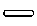
\includegraphics[height=20pt]{diagrams/CCSD_dE/CCSD_dE-figure3.pdf}}}.  The connected terms can then be characterized by their excitation type such that $\Top_{k}$ corresponds to $\ph{k}{k}$ excitations.

The $\Top_{1}$ operator represents the class of all connected $\ph{1}{1}$ MBPT diagrams, which are determined by the number of particle-hole pairs (or pair of up- and down-lines) at the top of the diagram,
\begin{align} \label{eq:t1_def}
  \Top_{1}\refket \equiv \sdiagram{CC_Amps/CC_Amps-figure0} &= \left(\Top^{(1)}_{1} + \Top^{(2)}_{1} + \cdots\right)\refket = \sdiagram{MBPT_linked/MBPT_linked-figure0} + \sdiagram{MBPT_linked/MBPT_linked-figure4} + \sdiagram{MBPT_linked/MBPT_linked-figure8} \notag \\
  &+ \sdiagram{MBPT_linked/MBPT_linked-figure10} + \sdiagram{MBPT_linked/MBPT_linked-figure11} + \sdiagram{MBPT_linked/MBPT_linked-figure16} + \sdiagram{MBPT_linked/MBPT_linked-figure17} + \cdots,
\end{align}
where only first-order $\Top^{(1)}$ and second-order $\Top^{(2)}$ terms are shown while resolvant lines and labels are removed for clarity.
The $\Top_{2}$ operator similarly represents the class of all connected $\ph{2}{2}$ MBPT diagrams.  The first- and second-order terms that belong to this class are,
\begin{align} \label{eq:t2_def}
  \Top_{2}\refket \equiv \sdiagram{CC_Amps/CC_Amps-figure1} &= \left(\Top^{(1)}_{2} + \Top^{(2)}_{2} + \cdots\right)\refket = \sdiagram{MBPT_linked/MBPT_linked-figure1} + \sdiagram{MBPT_linked/MBPT_linked-figure2} + \sdiagram{MBPT_linked/MBPT_linked-figure3} \notag \\
  &+ \sdiagram{MBPT_linked/MBPT_linked-figure6} + \sdiagram{MBPT_linked/MBPT_linked-figure7} + \sdiagram{MBPT_linked/MBPT_linked-figure13} + \sdiagram{MBPT_linked/MBPT_linked-figure14} + \sdiagram{MBPT_linked/MBPT_linked-figure15} + \cdots.
\end{align}
Additionally, the $\Top_{3}$ operator represents the class of all connected $\ph{3}{3}$ MBPT diagrams, of which there is only two second-order terms,
\begin{align}
  \Top_{3}\refket \equiv \sdiagram{CC_Amps/CC_Amps-figure2} &= \left(\Top^{(2)}_{3} + \cdots\right)\refket = \sdiagram{MBPT_linked/MBPT_linked-figure18} + \sdiagram{MBPT_linked/MBPT_linked-figure19} + \cdots.
\end{align}
So far, this is merely a redefinition of the connected class of MBPT diagrams up to all orders and is not particularly useful.  But the disconnected diagrams, neglected up to this point, can be recombined using the factorization theorem \ref{section:factorization_theorem} to provide a powerful simplification (see \cite{SHAVITT2009} for a more thorough derivation).

As an example, the remaining disconnected first- and second-order diagrams can be written as the product of connected diagrams.  First, the second-order disconnected diagram from the term $\fop^{2}\refket$ can be rewritten by adding a duplicate with the left and right subdiagrams exchanged, which doesn't change the value because the state labels are generic.  Then, the two disconnected diagrams can be rewritten using the factorization theorem following the example of Eq.\ \eqref{eq:factorization2},
\begin{equation}
  \xdiagram{MBPT/MBPT-figure12} = \frac{1}{2}\left( \xdiagram{MBPT/MBPT-figure12} + \xdiagram{MBPT/MBPT-figure13} \right) = \frac{1}{2}\left( \xdiagram{MBPT/MBPT-figure0} \right)^{2}.
\end{equation}
The resulting product involves the first-order component of the $\Top_{1}$ operator in Eq.\ \eqref{eq:t1_def}, $\Top^{(1)}_{1}$.  Algebraicly, this process is written below,
\begin{align} \label{eq:t1_factorization}
  \sum_{\mathclap{abij}}\frac{\fint{a}{i}\fint{b}{j}}{\Edenom{ab}{ij}\Edenom{a}{i}}\ket{\Phi^{ab}_{ij}} &= \frac{1}{2}\sum_{\mathclap{abij}}\frac{\fint{a}{i}\fint{b}{j}}{\Edenom{ab}{ij}\Edenom{a}{i}}\ket{\Phi^{ab}_{ij}} + \frac{1}{2}\sum_{\mathclap{abij}}\frac{\fint{a}{i}\fint{b}{j}}{\Edenom{ab}{ij}\Edenom{b}{j}}\ket{\Phi^{ab}_{ij}} = \frac{1}{2}\sum_{\mathclap{abij}}\fint{a}{i}\fint{b}{j}\frac{\Edenom{b}{j} + \Edenom{a}{i}}{\Edenom{ab}{ij}\Edenom{a}{i}\Edenom{b}{j}}\ket{\Phi^{ab}_{ij}} \notag \\
  &= \frac{1}{2}\left(\sum_{\mathclap{ai}}\frac{\fint{a}{i}}{\Edenom{a}{i}}\ket{\Phi^{a}_{i}}\right)\left(\sum_{\mathclap{bj}}\frac{\fint{b}{j}}{\Edenom{b}{j}}\ket{\Phi^{b}_{j}}\right) = \frac{1}{2}\left(\Top^{(1)}_{1}\right)^{2}.
\end{align}

This procedure can be repeated for the single second-order disconnected term from $\Vop^{2}\refket$,
\begin{align}
  \xdiagram{MBPT/MBPT-figure21} &= \frac{1}{2}\left( \xdiagram{MBPT/MBPT-figure21} + \xdiagram{MBPT/MBPT-figure22} \right) \notag \\
  &\hspace{140pt} = \frac{1}{2}\left( \xdiagram{MBPT/MBPT-figure1} \right)^{2}.
\end{align}
A similar results gives the product involving the first-order component of the $\Top_{2}$ operator in Eq.\ \eqref{eq:t2_def}, $\Top^{(1)}_{2}$.  Again, the factorization process is written algebraicly,
\begin{align} \label{eq:t2_factorization}
  \frac{1}{16}\sum_{\mathclap{\substack{abcd \\ ijkl}}}\frac{\vint{ab}{ij}\vint{cd}{kl}}{\Edenom{abcd}{ijkl}\Edenom{ab}{ij}}\ket{\Phi^{abcd}_{ijkl}} &= \frac{1}{32}\sum_{\mathclap{\substack{abcd \\ ijkl}}}\frac{\vint{ab}{ij}\vint{cd}{kl}}{\Edenom{abcd}{ijkl}\Edenom{ab}{ij}}\ket{\Phi^{abcd}_{ijkl}} + \frac{1}{32}\sum_{\mathclap{\substack{abcd \\ ijkl}}}\frac{\vint{ab}{ij}\vint{cd}{kl}}{\Edenom{abcd}{ijkl}\Edenom{cd}{kl}}\ket{\Phi^{abcd}_{ijkl}} \notag \\
  &= \frac{1}{32}\sum_{\mathclap{\substack{abcd \\ ijkl}}}\vint{ab}{ij}\vint{cd}{kl}\frac{\Edenom{cd}{kl} + \Edenom{ab}{ij}}{\Edenom{abcd}{ijkl}\Edenom{ab}{ij}\Edenom{cd}{kl}}\ket{\Phi^{abcd}_{ijkl}} \notag \\
  &= \frac{1}{2}\left(\frac{1}{4}\sum_{\mathclap{abij}}\frac{\vint{ab}{ij}}{\Edenom{ab}{ij}}\ket{\Phi^{ab}_{ij}}\right)\left(\frac{1}{4}\sum_{\mathclap{cdkl}}\frac{\vint{cd}{kl}}{\Edenom{cd}{kl}}\ket{\Phi^{cd}_{kl}}\right) = \frac{1}{2}\left(\Top^{(1)}_{2}\right)^{2}.
\end{align}

Lastly, for the disconnected terms from $\Vop\fop\refket$ and $\fop\Vop\refket$, the first duplication step can be skipped and the diagrams can be factorized following the procedure in Eq.\ \eqref{eq:factorization2},
\begin{equation}
  \xdiagram{MBPT/MBPT-figure5} + \xdiagram{MBPT/MBPT-figure9} = \xdiagram{MBPT/MBPT-figure29}.
\end{equation}
This factorization results in a mixed term between the the first-order components from the $\Top_{1}$ and $\Top_{2}$ operators,
\begin{align} \label{eq:t1t2_factorization}
  \frac{1}{4}\sum_{\mathclap{\substack{abc \\ ijk}}}\frac{\vint{ab}{ij}\fint{c}{k}}{\Edenom{abc}{ijk}\Edenom{ab}{ij}}\ket{\Phi^{abc}_{ijk}} &+ \frac{1}{4}\sum_{\mathclap{\substack{abc \\ ijk}}}\frac{\vint{ab}{ij}\fint{c}{k}}{\Edenom{abc}{ijk}\Edenom{c}{k}}\ket{\Phi^{abc}_{ijk}} = \frac{1}{4}\sum_{\mathclap{\substack{abcd \\ ijkl}}}\vint{ab}{ij}\fint{c}{k}\frac{\Edenom{c}{k} + \Edenom{ab}{ij}}{\Edenom{abc}{ijk}\Edenom{ab}{ij}\Edenom{c}{k}}\ket{\Phi^{abc}_{ijk}} \notag \\
  &= \left(\sum_{\mathclap{ck}}\frac{\fint{c}{k}}{\Edenom{c}{k}}\ket{\Phi^{c}_{k}}\right)\left(\frac{1}{4}\sum_{\mathclap{abij}}\frac{\vint{ab}{ij}}{\Edenom{ab}{ij}}\ket{\Phi^{ab}_{ij}}\right) = \Top^{(1)}_{1}\Top^{(1)}_{2}
\end{align}

Adding these factorized contributions from Eqs.\ \eqref{eq:t1_factorization}, \eqref{eq:t2_factorization}, and \eqref{eq:t1t2_factorization} gives $\frac{1}{2}\left(\Top^{(1)}_{1}\right)^{2} + \Top^{(1)}_{1}\Top^{(1)}_{2} + \frac{1}{2}\left(\Top^{(1)}_{2}\right)^{2} = \frac{1}{2}\left(\Top^{(1)}_{1} + \Top^{(1)}_{2}\right)^{2}$.  Repeating this procedure for all diagrams with two disconnected parts ($\mathrm{L}=2$) adds similar terms of all orders. The final contribution from the $\mathrm{L}=2$ class of diagrams with two disconnected parts is,
\begin{equation}
  \sum_{n=0}^{\infty}\left[\hat{R}_{0}\mathop{(\hat{V} - \Delta E_{0})}\right]^{n}\refket_{\mathrm{L=2}} = \frac{1}{2}\Top^{2}.
\end{equation}
A similar form results from any class of diagrams with $k$ disconnected pieces,
\begin{equation}
  \sum_{n=0}^{\infty}\left[\hat{R}_{0}\mathop{(\hat{V} - \Delta E_{0})}\right]^{n}\refket_{\mathrm{L=}k} = \frac{1}{k!}\Top^{k}.
\end{equation}

Therefore, summing over all classes of diagrams gives the final result that justifies the exponential ansatz,
\begin{equation}
  \ket{\Psi} = \sum_{k=0}^{\infty}\sum_{n=0}^{\infty}\left[\hat{R}_{0}\mathop{(\hat{V} - \Delta E_{0})}\right]^{n}\refket_{\mathrm{L=}k} = \sum_{k=0}^{\infty}\frac{1}{k!}\Top^{k}\refket = \E^{\Top}\refket.
\end{equation}
This equation shows the true strength and elegance of coupled cluster theory.  By an ingenious reorganization and factorization of certain MBPT diagrams, the exponential ansatz captures the contribution of these excitations to infinite order.  A more comprehensive derivation of the linked-cluster theorem can by found in \cite{SHAVITT2009}.

\section{Example: Pairing Model} \label{section:pairingmodel}

It's beneficial to illustrate a simplified example of coupled cluster theory.  For this purpose, we turn our attention to the simple pairing model.  This system uses a model space of $N$ shells, or degenerate groups of single-particle states, each with two opposite spin orbitals.
\begin{figure}[h]
  \centering
  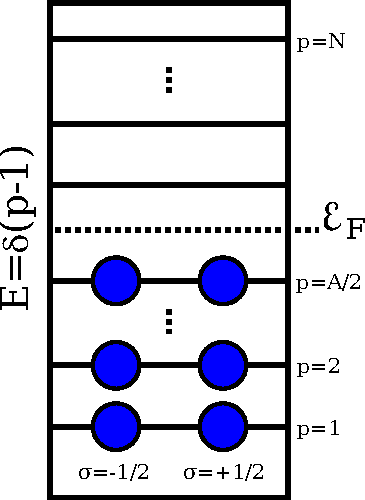
\includegraphics[width=0.35\linewidth]{CC/Pairing_Space.pdf}
  \caption{Schematic representation of the pairing model space.  The shells are equally spaced and doubly degenerate with one spin-up and one spin-down state.}
  \label{fig:pairing_space}
\end{figure}

With a closed-shell reference state, the Hamiltonian is restricted to interact only between unbroken pairs, which can be written as,
\begin{gather} \label{eq:pairing_ham}
  \HamB{1} = \delta \sum_{p}^{N} \mathop{(p-1)} \left[ \co{p_{+}}\ao{p_{+}} +\ \co{p_{-}}\ao{p_{-}} \right],\ \ \text{and} \notag \\
  \HamB{2} = -\frac{g}{2} \sum_{pq}^{N} \co{p_{+}}\co{p_{-}}\ao{q_{-}}\ao{q_{+}},
\end{gather}
where $\delta$ and $g$ are free parameters and the $\pm$ labels represent the spin-up and spin-down states, respectively.

As with all other coupled cluster calculations in this work, the first step is transforming the problem to the Hartree-Fock basis.  In this case, the restriction to unbroken pairs means that the original single-particle states do not mix with states in other shells.  In fact, the original basis is already an eigenbasis of the Fock operator, Eq.\ \eqref{eq:fock_operator}, so that all is left of the HF transformation is to redefine the single-particle energies to their corresponding Hartree-Fock energies while the two-body interaction is left unchanged,
\begin{gather}\label{eq:pairing_hf}
  \varepsilon_{p_{m_{p}}} = \Hint{1}{p_{m_{p}}}{p_{m_{p}}} + \sum_{im_{i}}\Hint{2}{p_{m_{p}}i_{m_{i}}}{p_{m_{p}}i_{m_{i}}} = \delta\mathop{(p-1)} - \frac{g}{2} \notag \\
  \vint{pq}{rs} = \Hint{2}{pq}{rs}
\end{gather}
Again, because of the pairing restriction, only hole-state energies have to be redefined.

The next step in calculating the ground-state correlation energy is to solve the CCD equations in the Hartree-Fock basis.  The system of equations comes from the terms of Eq.\ \eqref{eq:ccsd2} that contain only the $\Top_{2}$ operator, and are most easily derived with diagrammatic techniques, see \cite{SHAVITT2009}.
\begin{gather} \label{eq:ccd_equations}
  \statebra{ab}{ij}\mathop{(\Ham\E^{\Top_{2}})_{\text{C}}}\refket\ - \diagram{CCSD_t2/CCSD_t2-figure2} - \diagram{CCSD_t2/CCSD_t2-figure1} = \diagram{CCSD_t2/CCSD_t2-figure0} \notag \\[-1.5ex]
  + \diagram{CCSD_t2/CCSD_t2-figure5} + \diagram{CCSD_t2/CCSD_t2-figure6} + \diagram{CCSD_t2/CCSD_t2-figure7} + \diagram{CCSD_t2/CCSD_t2-figure11} \notag \\[-1.5ex]
  + \diagram{CCSD_t2/CCSD_t2-figure12} + \diagram{CCSD_t2/CCSD_t2-figure13} + \diagram{CCSD_t2/CCSD_t2-figure14} \notag \\
  \mathop{(\varepsilon_{i} + \varepsilon_{j} - \varepsilon_{a} - \varepsilon_{b})}\tamp{ab}{ij} = \vint{ab}{ij} + \frac{1}{2}\sum\limits_{\mathclap{kl}}\vint{kl}{ij}\tamp{ab}{kl} + \frac{1}{2}\sum\limits_{\mathclap{cd}}\vint{ab}{cd}\tamp{cd}{ij} - \Perm{ij|ab}\sum\limits_{\mathclap{kc}}\vint{kb}{ic}\tamp{ac}{kj} \notag \\
  + \frac{1}{4}\sum\limits_{\mathclap{klcd}}\vint{kl}{cd}\tamp{ab}{kl}\tamp{cd}{ij} + \Perm{ab}\sum\limits_{\mathclap{klcd}}\vint{kl}{cd}\tamp{ac}{lj}\tamp{bd}{ki} - \Perm{ij}\frac{1}{2}\sum\limits_{\mathclap{klcd}}\vint{kl}{cd}\tamp{ab}{lj}\tamp{cd}{ki} - \Perm{ab}\frac{1}{2}\sum\limits_{\mathclap{klcd}}\vint{kl}{cd}\tamp{db}{ij}\tamp{ca}{kl}
\end{gather}
The CCD equations are written in this particular form so that an initial guess for all the amplitudes $\tamp{ab}{ij}$ can be used to calculate the right-hand side of Eq.\ \eqref{eq:ccd_equations} and update the amplitudes on the left-hand side iteratively until the amplitudes do not change within a certain tolerance.

Lastly, the CCD correlation energy can be found with the $\Top_{2}$ term of Eq.\ \eqref{eq:cc_schrodeq},
\begin{equation} \label{eq:ccd_energy}
  \Ecorr_{\text{CCD}} = \refbra\mathop{(\Ham\E^{\Top_{2}})_{\text{C}}}\refket\ = \diagram{CCSD_dE/CCSD_dE-figure0}\ =\ \frac{1}{4}\sum\limits_{\mathclap{klcd}}\vint{kl}{cd}\tamp{cd}{kl}
\end{equation}
The correlation energies for a specific case, with $\delta = 1.0$, $N = 4$, and $A = 4$, were calculated for a number of different interaction strengths, $g$.  The results are shown in Fig.\ \ref{fig:pairingplot} along with the MBPT correlation energies to third (MBPT3) and fourth (MBPT4) orders for comparison.  The MBPT expressions for second and third order are,
\begin{align} \label{eq:mbpt_2_3}
  \Ecorr_{\text{MBPT2}} &= \frac{1}{4}\sum\limits_{\mathclap{ijab}}\frac{\vint{ij}{ab}\vint{ab}{ij}}{\Edenom{ab}{ij}}, \\
  \Ecorr_{\text{MBPT3}} &= \Ecorr_{\text{MBPT2}} + \frac{1}{8}\sum\limits_{\mathclap{ijabcd}}\frac{\vint{ij}{ab}\vint{ab}{cd}\vint{cd}{ij}}{\Edenom{ab}{ij}\Edenom{cd}{ij}} + \frac{1}{8}\sum\limits_{\mathclap{ijklab}}\frac{\vint{ij}{ab}\vint{kl}{ij}\vint{ab}{kl}}{\Edenom{ab}{ij}\Edenom{ab}{kl}}.
\end{align}
Generally, the fourth-order expression contains 39 additional terms.  However, most of these vanish in this case because of the form of the pairing interaction.

\begin{figure}[h]
  \centering
  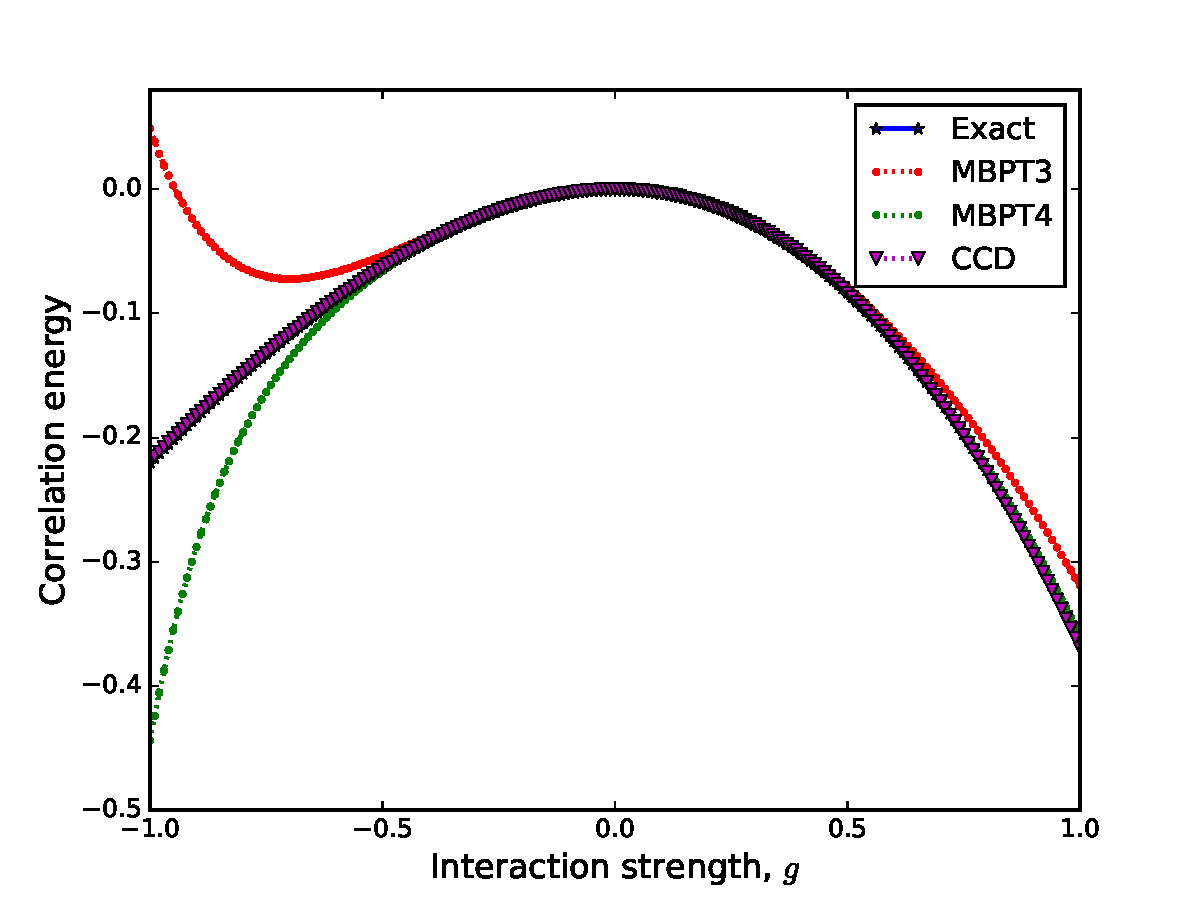
\includegraphics[width=0.8\textwidth]{CC/CCDMBPT4theory.pdf}
  \caption{Correlation energy for the pairing model with exact diagonalization, CCD, and perturbation theory to third (MBPT3) and fourth order (MBPT4) for a range of interaction values, $g$.}
  \label{fig:pairingplot}
\end{figure}

Also shown are the exact results from the CI method.  With an example this small, it's possible to diagonalize, and even show explicitly, the full CI Hamiltonian matrix for an exact result.  There are six possible Slater determinants with no broken pairs, one representing the reference state, four representing various $\ph{2}{2}$ excitations, one representing a $\ph{4}{4}$ excitation.  The diagonal elements of the matrix include the single-particle energies of the constituent states, and the matrix elements between Slater determinants with no overlap vanish in accordance with the Slater-Condon rules, see Eq.\ \eqref{eq:slater_condon} and \cite{SLATER1929,CONDON1930}.  The full Hamiltonian matrix to be diagonalized is,
\begin{equation}
  H = \begin{bmatrix}
    2\delta -g & -g/2 & -g/2 & -g/2 & -g/2 & 0 \\ -g/2 & 4\delta -g &
    -g/2 & -g/2 & -0 & -g/2 \\ -g/2 & -g/2 & 6\delta -g & 0 & -g/2 &
    -g/2 \\ -g/2 & -g/2 & 0 & 6\delta-g & -g/2 & -g/2 \\ -g/2 & 0 & -g/2
    & -g/2 & 8\delta-g & -g/2 \\ 0 & -g/2 & -g/2 & -g/2 & -g/2 &
    10\delta -g
  \end{bmatrix}.
\end{equation}

As methods to obtain the ground-state correlation energy, both CI and CC decouple, to some degree, the reference state and excitations from it.  This decoupling has the effect of shuffling correlations into the reference state and suppressing matrix elements connected to it.  Full decoupling between the reference state and all other Slater determinants can only be achieved with untruncated versions of these techniques, while decoupling of the strongest correlations can be approximately obtained with appropriate truncations.  However, unlike other many-body methods, the most unique aspect of the CC similarity transformation is that because of its non-unitarity, the resulting Hamiltonian will not be Hermitian.  This decoupling and non-Hermiticity can be seen in Fig.\ \ref{fig:pairingmatrix}, which shows the effect of the CC similarity transformation on the Hamiltonian for a pairing case with $N = 6$ and $A = 4$.
\begin{figure}[h]
  \centering
  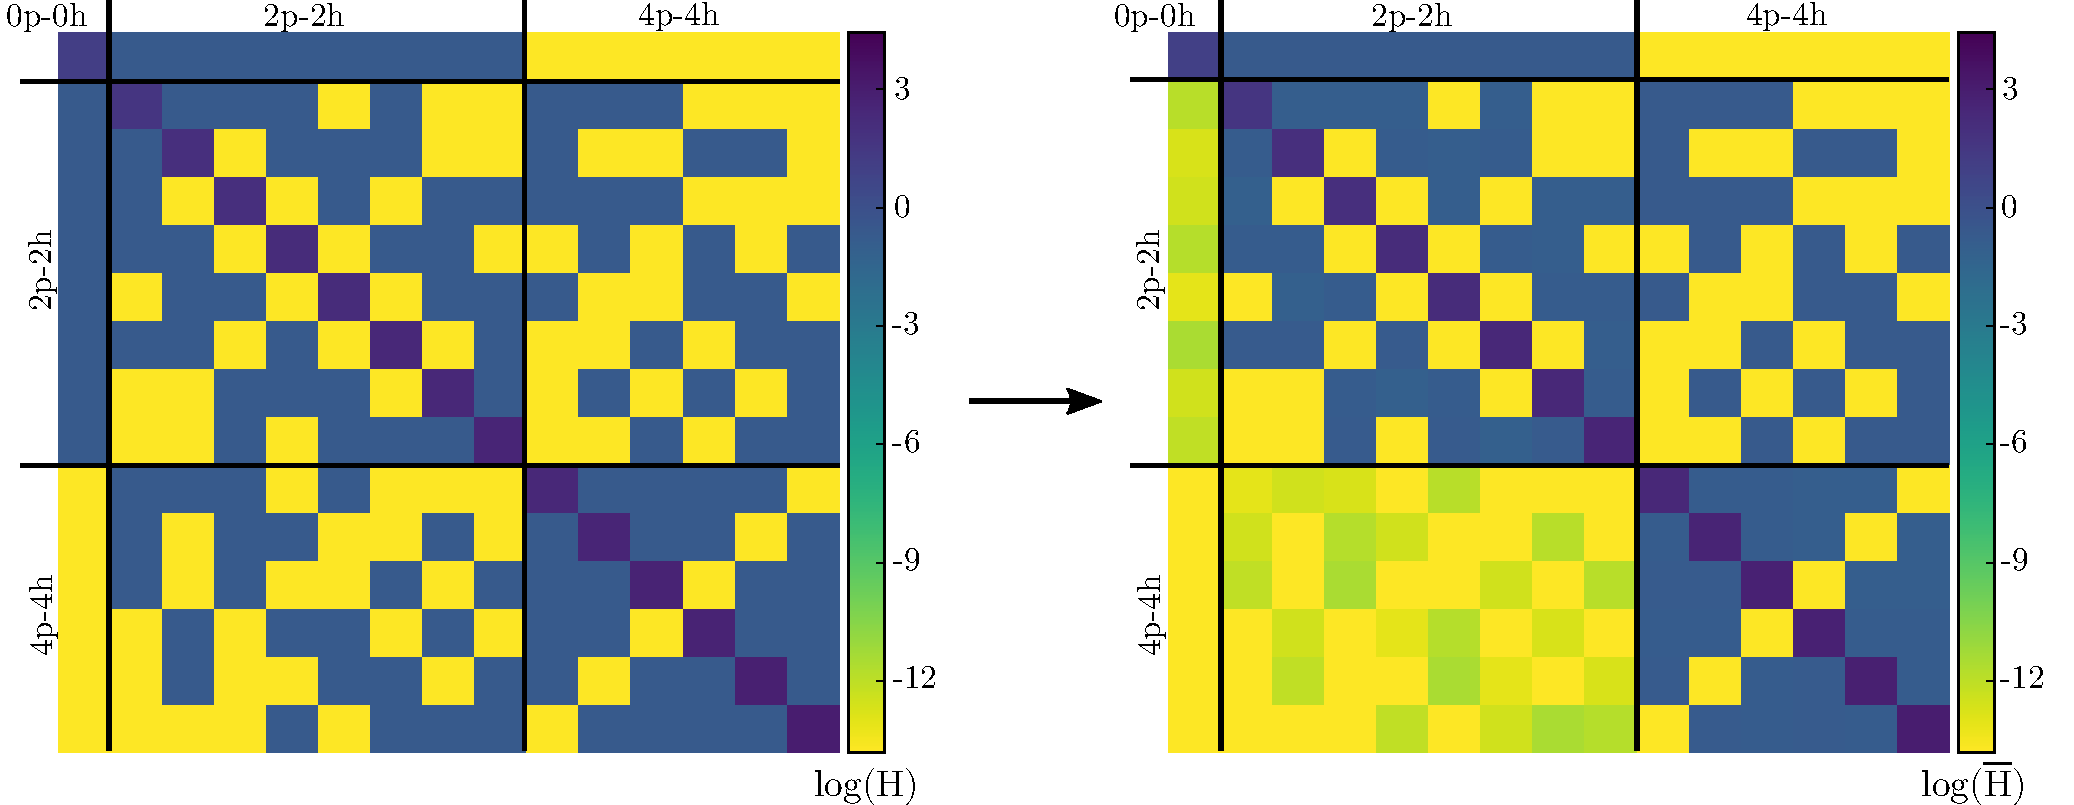
\includegraphics[width=\textwidth]{CC/pairingmatrix.pdf}
  \caption{Visualization of the CCD similarity transform on the pairing Hamiltonian for four particles and six shells.  This shows the main function of CCD, which is to decouple $\ph{2}{2}$ excitations from the ground state, shown by the suppression of matrix elements on the first column. In the pairing model, this also has the effect of decoupling $\ph{2}{2}$ excitations from $\ph{4}{4}$ excitations.  Also, the non-unitary nature of the transformation is obvious given the asymmetry of the resulting Hamiltonian.}
  \label{fig:pairingmatrix}
\end{figure}
The effective Hamiltonian $\EHam$ shown in Fig.\ \ref{fig:pairingmatrix} can be explicitly built, and it happens to be beneficial to do so as part of most CC calculations, both for solving the CC equations and for use in post-CC methods.  This topic is discussed in detail in the next section.




\section{Solving the Coupled Cluster Equations} \label{section:solvingcc}

As described above, the coupled cluster equations are solved by first initializing all of the cluster amplitudes, then updating them by computing various sums over particle and hole combinations, $\text{CC}\mathop{(\Top)}$.  This updating procedure is performed over multiple iterations until the amplitudes stay unchanged within a certain tolerance.
\begin{align} \label{eq:cc_algorithm}
  &\text{Initialize}:&    \hspace{-20pt}&\Top^{\mathop{(0)}} = \Top_{\text{init}} \notag \\
  &\text{Iterate}:&       \hspace{-20pt}&\Top^{\mathop{(n+1)}}\ \leftarrow\ \text{CC}\mathop{(\Top^{\mathop{(n)}})}
\end{align}

Generally, the convergence of this algorithm depends on the relative magnitudes between the inter-particle force and the single-particle energy spacing.  For a relatively small Fermi gap between the closed shell of occupied states and the unoccupied particle states, the energy denominators will approach zero and cause a divergent or chaotic solution \cite{SZAKACS2008}.  Physically, this situation occurs when a system exhibits strong many-particle clustering, which is difficult to capture with only the single and double excitations of CCSD.  A simple way to avoid this ill-defined behavior is to scale the energy denominators for early iterations or to employ linear mixing to dampen the solution.
\begin{equation} \label{eq:cc_damping}
  \Top^{\mathop{(n+1)}} \leftarrow\ \alpha\text{CC}\mathop{(\Top^{\mathop{(n)}})} + \left(1 - \alpha\right)\Top^{\mathop{(n)}}
\end{equation}
If a solution to a highly-collective system does not diverge, it typically converges very slowly.  To improve the convergence rate, techniques already utilized for the Hartree-Fock iterations can also be employed here, such as DIIS \cite{PULAY1980393,PULAY1982556} or Broyden's method \cite{BROYDEN1965557}.  The additional computational complexity for the CC iterations is simply a multiplicative factor equal to the number of iterations performed.  Typical calculations in this work with DIIS acceleration are converged within $\sim 30$ iterations.  Therefore, any significant improvements to the CC algorithm will involve the expensive sums embedded within the function $\text{CC}\mathop{(\Top^{\mathop{(n)}})}$.


\subsection{Symmetry Channels} \label{section:symmetry_channels}

For the coupled cluster equations, as well as many other many-body methods, the first way to simplify the various sums is to exploit any symmetries of the underlying Hamiltonian of a particular problem.  These symmetries manifest as conserved quantities, and because of the underlying nature of the cluster operators, see Section\ \ref{section:linkedcluster}, these must conserve these quantum numbers as well.  For example, the pairing Hamiltonian of Section\ \ref{section:pairingmodel} has a symmetry that conserves both the total spin projection and the number of pairs.  The Coulomb Hamiltonian of Section\ \ref{section:electrongas}, which has translational symmetry, conserves the linear momentum of any state.  Finally, the spherical symmetry of the nuclear Hamiltonian ensures that angular momentum and parity are conserved.  To utilize these symmetries, any sums that contain many-body states with different conserved quantum numbers can be ignored.  For efficiency, these symmetry groups can be pre-sorted into \textit{channels}, $\Sigma_{\vec{\xi}}$, where $\vec{\xi}$ represents the relevant quantum numbers of a certain channel.

For CCSD calculations, useful types of channels include the direct two-body channels, $\Sigma_{\vec{\xi}_{1}}$--which categorizes the vector sum of two single-particle-state quantum numbers--and the cross two-body channels, $\Sigma_{\vec{\xi}_{2}}$--which categorizes the vector difference of two single-particle-state quantum numbers or, equivalently, the vector sum of a the quantum numbers of a single-particle state and a time-reversed single-particle state.
\begin{gather}
  \vec{\xi}_{pq} = \vec{\xi}_{p} + \vec{\xi}_{q}\ \ \longrightarrow\ \ \ket{pq} \in \Sigma_{\vec{\xi}_{1}=\vec{\xi}_{pq}} \\
  \vec{\xi}_{p\bar{q}} = \vec{\xi}_{p} - \vec{\xi}_{q} = \vec{\xi}_{p} + \vec{\xi}_{\bar{q}}\ \ \longrightarrow\ \ \ket{p\bar{q}} \in \Sigma_{\vec{\xi}_{2}=\vec{\xi}_{p\bar{q}}}
\end{gather}
Also useful is the one-body channels, $\Sigma_{\vec{\xi}_{3}}$, which categorizes both single-particle states by their conserved quantum numbers.  These one-body channels can also characterize a special type of three-body state: the vector difference between the quantum numbers of a direct two-body state and a single-particle state or, equivalently, the vector sum of the quantum numbers of a two-body direct state and a time-reversed single-particle state,
\begin{gather}
  \vec{\xi}_{p}\ \ \longrightarrow\ \ \ket{p} \in \Sigma_{\vec{\xi}_{3}=\vec{\xi}_{p}} \\
  \vec{\xi}_{pq\bar{r}} = \vec{\xi}_{p} + \vec{\xi}_{q} - \vec{\xi}_{r} = \vec{\xi}_{p} + \vec{\xi}_{q} + \vec{\xi}_{\bar{r}}\ \ \longrightarrow\ \ \ket{pq\bar{r}} \in \Sigma_{\vec{\xi}_{3}=\vec{\xi}_{pq\bar{r}}}.
\end{gather}

Using these channel structures, the interaction matrix elements and cluster amplitudes can be built in different ways.  The full applicability of these structures are shown in detail in the appendix \ref{chapter:appendix_computational}, but a few examples using sums in the CCD equations \eqref{eq:ccd_equations} are shown here.  The direct two-body channels can be used when two summed indices appear in the bra- or ket-state of multiple matrix-elements,
\begin{equation} \label{eq:channel_sums_1}
  \frac{1}{2}\sum\limits_{\mathclap{cd}}\vint{ab}{cd}\tamp{cd}{ij} = \frac{1}{2}\sum\limits_{\mathclap{\ket{cd}}}\vint{ab}{cd}\tamp{cd}{ij}\ \ \text{for}\ \ket{cd} \in \Sigma_{\vec{\xi}_{ab}}=\Sigma_{\vec{\xi}_{ij}}.
\end{equation}
The cross two-body channels are used when two summed indices appear in the opposite corresponding bra- and ket-states of multiple matrix-matrix elements,
\begin{equation} \label{eq:channel_sums_2}
  \sum\limits_{\mathclap{kc}}\vint{kb}{ic}\tamp{ac}{kj} = \sum\limits_{\mathclap{\ket{k\bar{c}}}}\vint{k\bar{c}}{i\bar{b}}\tamp{a\bar{j}}{k\bar{c}}\ \ \text{for}\ \ket{k\bar{c}} \in \Sigma_{\vec{\xi}_{i\bar{b}}}=\Sigma_{\vec{\xi}_{a\bar{j}}}.
\end{equation}
Lastly, the one- and three-body channels are used when a single summed index appears opposite a direct two-body state in multiple matrix elements,
\begin{equation} \label{eq:channel_sums_3}
  \frac{1}{2}\sum\limits_{\mathclap{klcd}}\vint{kl}{cd}\tamp{db}{ij}\tamp{ca}{kl} = \frac{1}{2}\sum\limits_{\mathclap{\substack{\ket{kl\bar{c}} \\ \ket{d}}}}\vint{kl\bar{c}}{d}\tamp{d}{ij\bar{b}}\tamp{a}{kl\bar{c}}\ \ \text{for}\ \ket{kl\bar{c}},\ket{d} \in \Sigma_{\vec{\xi}_{ij\bar{b}}}=\Sigma_{\vec{\xi}_{a}}.
\end{equation}


\subsection{Matrix Structures and Intermediates} \label{section:maxtrix_intermediates}

Symmetry channels not only provide an organized structure for the interaction matrix elements and cluster amplitudes, and remove any terms that violate the underlying symmetry of a problem, but they also naturally provide an efficient way of performing sums using matrix-matrix multiplications.  For example, the sums in Eqs.\ \eqref{eq:channel_sums_1}--\eqref{eq:channel_sums_3} can be reformulated as matrix-matrix multiplications by structuring the channel-separated interaction matrix elements and cluster amplitudes into individual matrices.  These operations can be performed very quickly using highly optimized linear algebra algorithms like those found in BLAS (Basic Linear Algebra Subprograms) \cite{blas}.  The matrices can be reordered so that the summed indices correspond to the internal columns and rows of those matrices.

For the direct two-body case of Eq.\ \eqref{eq:channel_sums_1}, the structures are already in the correct order such that the state $\ket{cd}$, indexed by the columns of $\bvint{}{}$ and the rows of $\btamp{}{}$, is summed by multiplying the two matrices,
\begin{equation} \label{eq:channel_matrices_1}
  \frac{1}{2}\sum\limits_{\mathclap{cd}}\vint{ab}{cd}\tamp{cd}{ij} = \frac{1}{2}\bvint{ab}{cd}\cdot\btamp{cd}{ij}\ \ \text{for}\ \ket{ab},\ket{ij},\ket{cd} \in \Sigma_{\vec{\xi}_{1}}.
\end{equation}
For the cross two-body case of Eq.\ \eqref{eq:channel_sums_2}, the states $\ket{j}$, $\ket{b}$, and $\ket{c}$ are time reversed so that the summed variables are collected in a state $\ket{k\bar{c}}$.  Then the matrix structures are reordered so this state is indexed by columns and rows of $\btamp{}{}$ and $\bvint{}{}$, respectively,
\begin{equation} \label{eq:channel_matrices_2}
  \sum\limits_{\mathclap{kc}}\vint{kb}{ic}\tamp{ac}{kj} = \btamp{a\bar{j}}{k\bar{c}}\cdot\bvint{k\bar{c}}{i\bar{b}}\ \ \text{for}\ \ket{a\bar{j}},\ket{i\bar{b}},\ket{k\bar{c}} \in \Sigma_{\vec{\xi}_{2}}.
\end{equation}
Lastly, for the case of Eq.\ \eqref{eq:channel_sums_3}, the states $\ket{b}$ and $\ket{c}$ are time-reversed so that the states $\ket{d}$ and $\ket{kl\bar{c}}$ appear in two different matrix elements.  Then, the matrix structures are reorganized so the summed states occur in the appropriate rows and columns for matrix-matrix multiplication,
\begin{equation} \label{eq:channel_matrices_3}
  \frac{1}{2}\sum\limits_{\mathclap{klcd}}\vint{kl}{cd}\tamp{db}{ij}\tamp{ca}{kl} = \frac{1}{2}\btamp{a}{kl\bar{c}}\cdot\bvint{kl\bar{c}}{d}\cdot\btamp{d}{ij\bar{b}}\ \ \text{for}\ \ket{a},\ket{ij\bar{b}},\ket{kl\bar{c}},\ket{d} \in \Sigma_{\vec{\xi}_{3}}.
\end{equation}

These sums correspond to different components of the updated cluster amplitudes according to Eq.\ \eqref{eq:cc_algorithm}.  So the different channel structures of the matrix-matrix multiplications correspond to different amplitude structures according to the sum's external indices.  The two external direct two-body states of Eq.\ \eqref{eq:channel_matrices_1}, $\ket{ab}$ and $\ket{ij}$, naturally map to the direct amplitude structure,
\begin{equation} \label{eq:amp_matrices_1}
  \btamp{ab}{ij}\ \leftarrow\ \frac{1}{2}\bvint{ab}{cd}\cdot\btamp{cd}{ij}\ \ \text{for}\ \ket{ab},\ket{ij},\ket{cd} \in \Sigma_{\vec{\xi}_{1}}.
\end{equation}
Similarly, the two external cross two-body states of Eq.\ \eqref{eq:channel_matrices_2}, $\ket{a\bar{j}}$ and $\ket{i\bar{b}}$, naturally map to the cross amplitude structure,
\begin{equation} \label{eq:amp_matrices_2}
  \btamp{a\bar{j}}{i\bar{b}}\ \leftarrow\ \btamp{a\bar{j}}{k\bar{c}}\cdot\bvint{k\bar{c}}{i\bar{b}}\ \ \text{for}\ \ket{a\bar{j}},\ket{i\bar{b}},\ket{k\bar{c}} \in \Sigma_{\vec{\xi}_{2}}.
\end{equation}
Lastly, the one- and three-body external states of of Eq.\ \eqref{eq:channel_matrices_3}, $\ket{a}$ and $\ket{i\bar{b}}$, naturally map to the one-body amplitude structure characterized by the index $a$,
\begin{equation} \label{eq:amp_matrices_3}
  \btamp{a}{ij\bar{b}}\ \leftarrow\ \frac{1}{2}\btamp{a}{kl\bar{c}}\cdot\bvint{kl\bar{c}}{d}\cdot\btamp{d}{ij\bar{b}}\ \ \text{for}\ \ket{a},\ket{ij\bar{b}},\ket{kl\bar{c}},\ket{d} \in \Sigma_{\vec{\xi}_{3}}.
\end{equation}

The last summation in the matrix-matrix form of Eqs.\ \eqref{eq:channel_matrices} and \eqref{eq:amp_matrices} involves two multiplications, which suggests the need for an \textit{intermediate} matrix to hold the result of the first operation.  This is the last main ingredient to an efficient CC algorithm.  To see the benefit of intermediate structures, it's helpful to examine an expensive sum from the CCD equations.  For typical calculations, particle states outnumber hole states by an order of magnitude, $n_{p} \sim 10n_{h}$, which means that one of the most expensive sums is,
\begin{equation}
  \frac{1}{4}\sum\limits_{\mathclap{klcd}}\vint{kl}{cd}\tamp{ab}{kl}\tamp{cd}{ij}.
\end{equation}
Because this term must be computed for each $\tamp{ab}{ij}$, its computational cost naively scales as $\mathcal{O}\left( N_{h}^{4}N_{p}^{4}\right)$.  However, using the matrix form of this sum and an intermediate matrix,
\begin{equation} \label{eq:intermediate}
  \frac{1}{4}\sum\limits_{\mathclap{klcd}}\vint{kl}{cd}\tamp{ab}{kl}\tamp{cd}{ij} = \frac{1}{4}\btamp{ab}{kl}\cdot\left(\bvint{kl}{cd}\cdot\btamp{cd}{ij}\right) = \frac{1}{4}\btamp{ab}{kl}\cdot\bxint{kl}{ij}\ \rightarrow\ \btamp{ab}{ij}.
\end{equation}
this term is now computed as the combination of two sums, each scaling as $\mathcal{O}\left( N_{h}^{4}N_{p}^{2}\right)$.  These intermediates can also be used as a way to combine similar sums.  For example, the last step of Eq.\ \ref{eq:intermediate} has a very similar structure to the first sum in Eq.\ \ref{eq:ccd_equations}.  Therefore, the two sums can be written with a common intermediate as,
\begin{gather} \label{eq:intermediate_2}
  \frac{1}{2}\sum\limits_{\mathclap{kl}}\vint{kl}{ij}\tamp{ab}{kl} + \frac{1}{4}\sum\limits_{\mathclap{klcd}}\vint{kl}{cd}\tamp{ab}{kl}\tamp{cd}{ij} = \frac{1}{2}\btamp{ab}{kl}\cdot\left[ \bvint{kl}{ij} + \frac{1}{2}\bvint{kl}{cd}\cdot\btamp{cd}{ij} \right] = \frac{1}{4}\btamp{ab}{kl}\cdot\bxint{kl}{ij}\ \rightarrow\ \btamp{ab}{ij}, \notag \\
  \text{where},\hspace{10pt} \bxint{kl}{ij} = \bvint{kl}{ij} + \frac{1}{2}\bvint{kl}{cd}\cdot\btamp{cd}{ij}
\end{gather}

It just so happens that this form of the intermediate $\xint{kl}{ij}$ is equivalent to the $\mathrm{hhhh}$ component of the CCD similarity transformed Hamiltonian, $\EHam$.  Constructing other intermediates in this way gives similar results, so it's a natural extension to actually construct the effective Hamiltonian at each iteration for the express purpose of using it as different intermediate components for the CC equations.  This has the added benefit of having already computed the effective Hamiltonian for post-CC methods.  The different components of the CCD effective Hamiltonian, $\EHam_{\mathrm{CCD}} = \left(\Ham\E^{\Top_{2}}\right)_{\mathrm{c}}$, are written below in both algebraic and diagrammatic form.  One-body components correspond to the vertex type \raisebox{-5pt}{\mbox{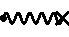
\includegraphics[height=20pt]{diagrams/CCSD_1b/CCSD_1b-figure23.pdf}}} and two-body terms correspond to the vertex type \raisebox{-5pt}{\mbox{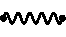
\includegraphics[height=20pt]{diagrams/CCSD_1b/CCSD_1b-figure24.pdf}}}.  The $\mathrm{pp}$, one-body component of $\EHam_{\mathrm{CCD}}$ is,
\begin{align} \label{eq:ccd_eff1}
  \diagram{CCSD_1b/CCSD_1b-figure3} &= \diagram{CCSD_1b/CCSD_1b-figure4} + \diagram{CCSD_1b/CCSD_1b-figure5} \notag \\
  \xint{a}{b} &= \fint{a}{b} - \frac{1}{2}\sum\limits_{klc}\vint{kl}{bc}\tamp{ac}{kl}.
\end{align}
The $\mathrm{hh}$, one-body component is,
\begin{align} \label{eq:ccd_eff2}
  \diagram{CCSD_1b/CCSD_1b-figure12} &= \diagram{CCSD_1b/CCSD_1b-figure9} + \diagram{CCSD_1b/CCSD_1b-figure10} \notag \\
  \xint{i}{j} &= \fint{i}{j} + \frac{1}{2}\sum\limits_{kcd}\vint{ik}{cd}\tamp{cd}{jk}.
\end{align}
The $\mathrm{hhhh}$, two-body component, which appears as the intermediate in Eqs.\ \eqref{eq:intermediate} and \eqref{eq:intermediate_2}, is,
\begin{align} \label{eq:ccd_eff3}
  \diagram{CCSD_2b/CCSD_2b-figure18} &= \diagram{CCSD_2b/CCSD_2b-figure19} + \diagram{CCSD_2b/CCSD_2b-figure20} \notag \\
  \xint{ij}{kl} &= \vint{ij}{kl} + \frac{1}{2}\sum\limits_{cd}\vint{ij}{cd}\tamp{cd}{kl}.
\end{align}
Lastly, the $\mathrm{hphp}$, two-body component is,
\begin{align} \label{eq:ccd_eff4}
  \diagram{CCSD_2b/CCSD_2b-figure34} &= \diagram{CCSD_2b/CCSD_2b-figure31} + \frac{1}{2}\fdiagram{CCSD_2b/CCSD_2b-figure36} \notag \\
  \xint{ia}{jb} &= \vint{ia}{jb} - \frac{1}{2}\sum\limits_{kc}\vint{ik}{cb}\tamp{ca}{jk}.
\end{align}

Using these terms, the CCD equations can be written in pseudo-linear form using the $\ph{2}{2}$ component of effective Hamiltonian form of the equations, Eq.\ \eqref{eq:ccsd1}.  This also explicitly shows the decoupling of the effective Hamiltonian with $\ph{2}{2}$ excitations.  The $\mathrm{pphh}$, two-body component, which should vanish when the CCS amplitudes have converged, is,
\begin{align} \label{eq:ccd_double_linear}
  \diagram{CCSD_2b/CCSD_2b-figure59} = 0 &= \diagram{CCSD_2b/CCSD_2b-figure60} + \diagram{CCSD_2b/CCSD_2b-figure61} + \diagram{CCSD_2b/CCSD_2b-figure62} \notag \\[-1.5ex]
  &+ \diagram{CCSD_t2/CCSD_t2-figure6} + \diagram{CCSD_2b/CCSD_2b-figure64} + \diagram{CCSD_2b/CCSD_2b-figure65} \notag \\
  \xint{ab}{ij} = 0 &= \vint{ab}{ij} + \Perm{ab}\sum\limits_{\mathclap{c}}\xint{a}{c}\tamp{cb}{ij} - \Perm{ij}\sum\limits_{\mathclap{k}}\xint{k}{i}\tamp{ab}{kj} \notag \\
  &+ \frac{1}{2}\sum\limits_{\mathclap{cd}}\xxint{ab}{cd}\tamp{cd}{ij} + \frac{1}{2}\sum\limits_{\mathclap{kl}}\xint{kl}{ij}\tamp{ab}{kl} - \Perm{ab|ij}\sum\limits_{\mathclap{kc}}\xint{kb}{ic}\tamp{ac}{kj}.
\end{align}
The components and intermediates of the CCSD effective Hamiltonian are much more complicated and are shown with their corresponding sums in the appendix \ref{chapter:appendix_diagrams}.




\section{Example: Homogeneous Electron Gas} \label{section:electrongas}

Another relatively simple calculation using the CCD approximation is the homogeneous electron gas.  This example aims to calculate the ground state energy of a three-dimensional gas of electrons subject to Coulomb repulsion.  This is an approximate model of the valence electrons in a metal, subject to a uniform background of positive charge from the nuclei and core electrons \cite{GROSS1991}.  As will be explained below, this calculation employs pure-momentum eigenstates such that $\ph{1}{1}$ excitations from the reference state are forbidden by momentum conservation.  This means that the problem reduces to the doubles approximation.  To obtain realistic results, a sufficiently-sized basis with a sufficient number of electrons must be used.  Therefore, the improvements discussed in Section \ref{section:solvingcc} are necessary to keep the computation time manageable as the system size increases.

With a uniform background potential, the electron gas can be constructed using eigenfunctions of the kinetic energy operator, $\HamB{1} = \Top = \frac{-\hbar^{2}}{2m}\nabla^{2}$.  In an infinite volume, however, there are an unlistable number of plane wave modes which satisfy this condition due to the continuous nature of the linear momentum eigenstates.  Therefore, the single-particle orbits will be constructed in a finite box of volume $\Omega$ and length $L$, and then the limit $L\rightarrow \infty$ can be taken after various expectation values have been computed.
\begin{gather} \label{eq:plane_wave}
  \frac{-\hbar^{2}}{2m}\nabla^{2}\phi_{\mathbf{k}\sigma}(\mathbf{r}) = \epsilon_{\mathbf{k}}\phi_{\mathbf{k}\sigma}(\mathbf{r}) \notag \\
  \phi_{\mathbf{k}\sigma}(\mathbf{r}) = \frac{1}{\sqrt{\Omega}}\exp{(i\mathbf{kr})}\xi_{\sigma}
\end{gather}
where $m$ is the electron mass, $\mathbf{k}$ is the wave number, and $\xi_{\sigma}$ is the spin function for either spin up or down electrons
\begin{equation}
  \xi_{\sigma=+1/2} = \left(\begin{array}{c} 1
    \\ 0 \end{array}\right) \hspace{0.5cm}
  \xi_{\sigma=-1/2} = \left(\begin{array}{c} 0 \\ 1 \end{array}\right).
\end{equation}

Assuming the single-particle orbits follow periodic boundary conditions within the containing box ($\phi(\mathbf{r}_{i}) = \phi(\mathbf{r}_{i} + L)$ for $i = x,y,z$) the wave numbers are quantized,
\begin{equation}
  k_{i} = \frac{2\pi n_{i}}{L}\hspace{0.5cm} i = x,y,z \hspace{0.5cm} n_{i} = 0, \pm 1, \pm 2, \dots
\end{equation}
A state can therefore be characterized by the quantum numbers $n_{x}$, $n_{x}$, and $n_{x}$ as well as the spin quantum number $\sigma$.  The energy of such a state, independent of the spin, can be written as
\begin{equation} \label{eq:infinite_energy}
  \epsilon_{n_{x}, n_{y}, n_{z}} = \frac{\hbar^2}{2m}\left(k_{x}^{2} + k_{y}^{2} + k_{z}^{2}\right) = \frac{\hbar^{2}}{2m}\left(\frac{2\pi }{L}\right)^{2} \left( n_{x}^{2} + n_{y}^{2} + n_{z}^{2}\right).
\end{equation}
\begin{figure}[h]
  \centering
  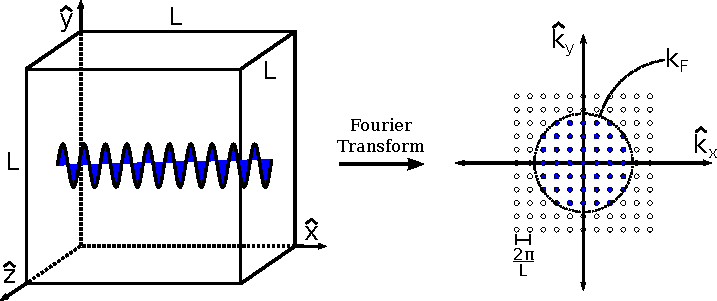
\includegraphics[width=\linewidth]{CC/Infinite_Space.pdf}
  \caption{Visulization of the Fourier transform of a finite box.  This transformation characterizes the construction of the single-particle basis for infinite matter, mapping plane waves in coordinate space onto finitely-spaced points in momentum space.}
  \label{fig:infinite_space}
\end{figure}

Now that the single-particle orbits are established, a particular basis consisting of these orbits can be chosen such that all states are included up to a closed shell.  This basis is then filled with electrons until a closed Fermi level is obtained.  Additionally, only the unpolarized case, in which all orbitals are occupied with one spin-up and one spin-down electron, will be considered here.  For this spherical-type level structure, the number of electrons required for closed shells increases quickly.  For example, the first six shells contain $2$, $14$, $38$, $54$, $66$ and $114$ states, respectively.

A finite number of electrons $A$ in a finite box of volume $\Omega$ naturally leads to the characterization of an infinite system by its number density density $\rho = A/\Omega$.  The average inter-electron distance, or \textit{Wigner-Seitz radius}, is defined as
\begin{equation} \label{wigner-seitz}
  \frac{4}{3}\pi r_{s}^{3} = \frac{1}{\rho},\hspace{0.5cm} r_{s} = \left(\frac{3}{4\pi\rho}\right)^{1/3}.
\end{equation}
In practice, these calculations are defined by the total number of shells included in the basis, the number of electrons, and the Wigner-Seitz radius, usually given in units of the Bohr radius, $r_{b} = \frac{\hbar}{mc\alpha}$, where $c$ is the speed of light and $\alpha$ is the fine-structure constant.

The last ingredient to this many-body calculation is the interaction between the electrons, the well-known Coulomb force.  Using atomic units, where the elementary charge $e = 1$ and the Coulomb constant $\frac{1}{4\pi\varepsilon_{0}} = 1$, this potential is simply
\begin{equation} \label{eq:coulomb}
  V\left( \mathbf{r}_{1}, \mathbf{r}_{2}\right) = \frac{1}{\lvert \mathbf{r}_{1} - \mathbf{r}_{2} \rvert}.
\end{equation}
As mentioned in chapter \ref{chapter:manybody}, this potential can be utilized in second-quantization by computing antisymmetrized integrals over the basis states.  In this case, the integrals have the form,
\begin{equation} \label{eq:coloumb_integral}
  \Hint{2}{pq}{rs} \equiv \int d\mathbf{r}_{1} d\mathbf{r}_{2}\  \phi^{*}_{\mathbf{k}_{p}\sigma_{p}}(\mathbf{r}_{1})\phi^{*}_{\mathbf{k}_{q}\sigma_{q}}(\mathbf{r}_{2}) \frac{1}{\lvert \mathbf{r}_{1} - \mathbf{r}_{2} \rvert} \left[\phi_{\mathbf{k}_{r}\sigma_{r}}(\mathbf{r}_{1})\phi_{\mathbf{k}_{s}\sigma_{s}}(\mathbf{r}_{2}) - \phi_{\mathbf{k}_{s}\sigma_{s}}(\mathbf{r}_{1})\phi_{\mathbf{k}_{r}\sigma_{r}}(\mathbf{r}_{2})\right].
\end{equation}
The symmetries of the Coulomb potential guarantee that the total linear momentum and total spin projection are conserved such that,
\begin{equation} \label{eq:coulomb-conserve}
  \mathbf{k}_{p} + \mathbf{k}_{q} = \mathbf{k}_{r} + \mathbf{k}_{s} \hspace{0.5cm} \text{and} \hspace{0.5cm} \sigma_{p} + \sigma_{q} = \sigma_{r} + \sigma_{s}.
\end{equation}
The integral is relatively simple given the form of the basis functions. The result is given in terms of the momentum transfer, $\mathbf{q}_{1} = \mathbf{k}_{p} - \mathbf{k}_{r}$ and $\mathbf{q}_{2} = \mathbf{k}_{p} - \mathbf{k}_{r}$,
\begin{equation} \label{eq:coulomb-int}
  \Hint{2}{pq}{rs} = \frac{4\pi \hbar c \alpha}{\Omega}\left[ \frac{\delta_{\sigma_{p}\sigma_{r}}\delta_{\sigma_{q}\sigma_{s}}}{\lvert \mathbf{q}_{1} \rvert^{2}} - \frac{\delta_{\sigma_{p}\sigma_{s}}\delta_{\sigma_{q}\sigma_{r}}}{\lvert \mathbf{q}_{2} \rvert^{2}} \right]
\end{equation}

The last preparation step before performing the coupled cluster algorithm is the Hartree-Fock transformation.  As with the pairing model, the single-particle orbitals are already eigenfunctions of the Fock operator, in this case because the translational invariance of the plane wave basis functions ensure that the HF terms of the form $\Hint{2}{pi}{qi}$ vanish due to momentum conservation, see Eq.\ \eqref{eq:fock_operator}.  Therefore, the HF transformation consists simply of redefining the single-particle energies while the two-body interaction is left unchanged.
\begin{gather}\label{eq:infinite_hf}
  \varepsilon_{p} = \epsilon_{\mathbf{k}_{p}} + \sum_{i}\Hint{2}{pi}{pi} \notag \\
  \vint{pq}{rs} = \Hint{2}{pq}{rs}
\end{gather}

As mentioned above, in the plane-wave basis, any single excitation from the reference state vanishes automatically due to momentum conservation so that $\tamp{a}{i} = 0$.  Therefore, it's necessary to include only double excitations (before adding triples, etc.).  Therefore, calculations for the electron gas use the pseudo-linear form of the CCD equations \eqref{eq:double_linear} and an effective Hamiltonian that excludes single excitations in Eqns.\ \eqref{eq:ccd_eff1}-\eqref{eq:eff4}.  To explore the HEG equation-of-state, the total energy per electron can be calculated as a function of the Wigner-Seitz radius.
\begin{figure}[h]
  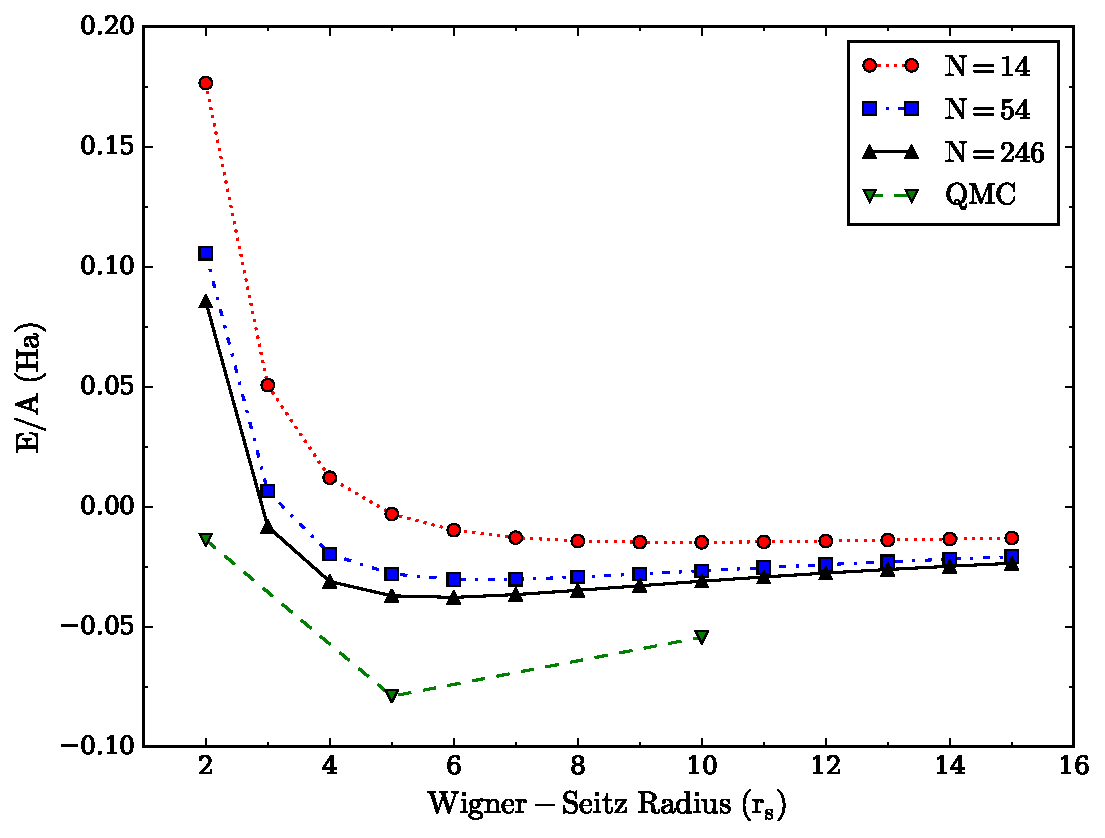
\includegraphics[width=\linewidth]{CC/Electronic_Gas.pdf}
  \caption{CCD energy per electron in Hartrees for the 3D homogeneous electron gas as function of the Wigner-Seitz radius in units of Bohr radii. The calculation used periodic boundary conditions and a basis with 25 shells, resulting in a total of $1238$ single-particle states. Also plotted are the variational quantum Monte Carlo (VMC) results from \cite{LOPEZ2006}.}  
  \label{fig:Electronic_Gas}
\end{figure}
In the limit $N,L \rightarrow \infty$, the plot in Fig.\ \ref{fig:Electronic_Gas} represents the equation-of-state for a 3D electron gas at absolute zero.  This curve can reveal many thermodynamic properties of the electron gas including the saturation density and saturation energy, which occur at the lowest point on the curve.  The CCD results are compared with the quasi-exact results from variational quantum Monte Carlo calculations from \cite{LOPEZ2006}.  The discrepancies between the saturation energies from the two methods can be partially attributed to an insufficient basis size.  However, even an appropriate extrapolation to an infinite basis won't be able to recover all of the required correlations, which suggests that CCSDT might be necessary.  Regardless of the value to the saturation energy, these CCD results do qualitatively reproduce the saturation radius at $r_{s} \approx 5.0$.



\section{Coupled Cluster for Finite Nuclei} \label{section:cc_nuclei}

The main purpose of this work is to calculate properties of atomic nuclei with coupled cluster theory.  From a many-body perspective, the main process is computing the converged cluster amplitudes and thus the important correlations of the system.  These amplitudes comprise the CC similarity transformation, which is versatile for constructing any effective operator, such as the Hamiltonian, that can act on the correlated system.  Therefore, the first step in calculating beta-decay properties of nuclei is solving for the ground-state wave function of specific closed-shell nuclei.


\subsection{Harmonic Oscillator Basis} \label{section:ho_basis}
Calculations of finite nuclei follow the basic structure of the algorithms used for the pairing model and the homogeneous electron gas, but they also differ in some significant ways.  Like the other examples, the first step is to construct a proper single-particle basis and reference state.  Because the nuclear Hamiltonian conserves angular momentum and parity, it's useful to construct orbits that are eigenfunctions of these operators.  For a system with no external potential, like the electron gas, this suggests a basis made of plane waves.  However, plane waves do not represent the bound states of a nucleus very well.  This property can be satisfied by introducing a fictitious external potential that mimics the mean field from the collection of nucleons.  Some phenomenological potentials, like the Woods-Saxon potential, properly consider the resonance and continuum states of realistic nuclei in addition to the bound states.  Many-body techniques discussed in this work have been applied to model spaces that include all three types of single-particle states \cite{MICHEL2006,HAGEN2007169} with some success.  However, for the many-body states considered in this work, it's sufficient to consider only bound single-particle states.  Therefore, the nuclear basis will be constructed from the isotropic harmonic oscillator,
\begin{equation}
  V\left(r\right) = \frac{1}{2}m\omega^{2}r^{2}.
\end{equation}

An eigenstate of the harmonic oscillator potential is defined by its principal quantum number $n$ and its orbital angular momentum quantum number $l$, which is denoted by the letters s, p, d, f... for the values $l=0,1,2,3...$ respectively.  Because of spin-orbit terms in the nuclear Hamiltonian, the orbital angular momentum is coupled to a particle spin to a total angular momentum of $j = \lvert \mathbf{l} + \mathbf{s} \rvert$, which results in a degeneracy of $2j + 1$ for each orbit.  This basis does not provide any simplification to eliminate single excitations, so CCSD will be used for all the following calculations.  A schematic version of this single-particle basis is shown in Fig.\ \ref{fig:Harmonic_Oscillator}.  The shell structure of this basis is characterized by the energy quantum numbers, $e = 2n + l$, of the HO single-particle spectrum.  This can be used to define the maximum-energy shell and the size of a HO basis with the parameter $e_{\mathrm{max}}$.
\begin{figure}[h]
  \centering
  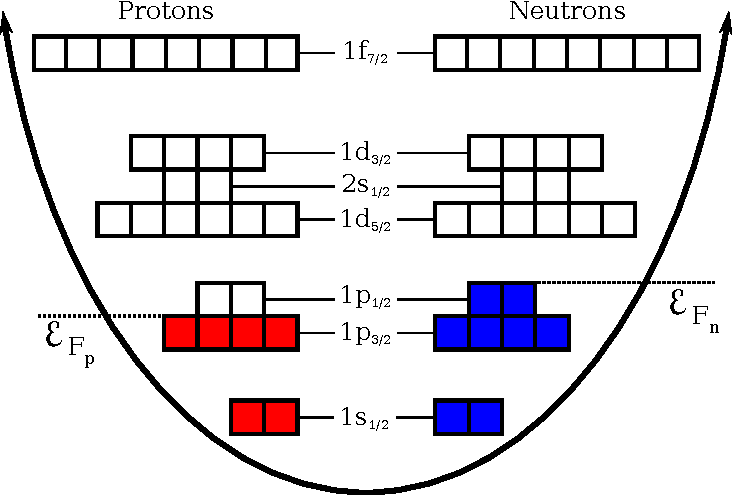
\includegraphics[width=0.6\linewidth]{CC/HO.pdf}
  \caption{A schematic illustration of the harmonic oscillator basis used for calculations of nuclei. Shown is an example of a initial reference state for carbon-14, with 6 protons filled to the p$3/2$-subshell closure and 8 neutrons filled to the p$1/2$-shell closure.  See text for details on the single-particle states.}
  \label{fig:Harmonic_Oscillator}
\end{figure}

One issue with this construction, is that while the single-particle orbits are eigenstates of the angular momentum operator and localized to the external potential, they are not translationally invariant, which is required by the nuclear Hamiltonian.  This means that there is a fictitious center-of-mass kinetic energy which must be removed from the Hamiltonian.  The COM kinetic energy can be written as the sum of one- and two-body pieces,
\begin{equation}
  \Top_{\mathrm{cm}} = \frac{\mathbf{P}_{\mathrm{cm}}}{2mA} = \sum^{A}_{pq}\frac{\mathbf{p}_{p}\cdot\mathbf{p}_{q}}{2mA} = \sum^{A}_{p}\frac{\mathbf{p}^{2}_{p}}{2mA} + \sum^{A}_{p<q}\frac{\mathbf{p}_{p}\cdot\mathbf{p}_{q}}{mA}.
\end{equation}
The one-body piece is just a scaled form of the original kinetic energy operator, and the two-body piece is given in a similar form to the original two-body Hamiltonian.  Both can be integrated into matrix elements like Eq.\ \eqref{eq:braket_integration},
\begin{gather} \label{eq:ke_integration}
    \KEint{1}{p}{q} \equiv \int d\mathbf{r}_{1}\  \phi^{*}_{p}\left(\mathbf{r}_{1}\right) \frac{\mathbf{p}^{2}_{1}}{2mA} \phi_{q}\left(\mathbf{r}_{1}\right), \notag \\
    \KEint{2}{pq}{rs} \equiv \int d\mathbf{r}_{1} d\mathbf{r}_{2}\  \phi^{*}_{p}\left(\mathbf{r}_{1}\right)\phi^{*}_{q}\left(\mathbf{r}_{2}\right) \frac{\mathbf{p}_{1}\cdot\mathbf{p}_{2}}{mA} \left[\phi_{r}\left(\mathbf{r}_{1}\right)\phi_{s}\left(\mathbf{r}_{2}\right) - \phi_{s}\left(\mathbf{r}_{1}\right)\phi_{r}\left(\mathbf{r}_{2}\right)\right].
\end{gather}
Subtracting the COM kinetic energy results in the \textit{intrinsic} Hamiltonian for finite nuclear systems,
\begin{align} \label{eq:intrinsic_hamiltonian}
  \Ham_{\mathrm{in}} = \left(1 - \frac{1}{A}\right)\sum_{\mathclap{pq}}\KEint{1}{p}{q}\ \co{p}\ao{q} &+ \frac{1}{4}\sum_{\mathclap{pqrs}}\left(\Hint{2}{pq}{rs} - \KEint{2}{pq}{rs}\right)\ \co{p}\co{q}\ao{s}\ao{r} \notag \\
  &+ \frac{1}{36}\sum_{\mathclap{pqrstu}}\Hint{3}{pqr}{stu}\ \co{p}\co{q}\co{r}\ao{u}\ao{t}\ao{s} + \cdots,
\end{align}
This form of the bare Hamiltonian (up to the three-body force) is used in the Hartree-Fock transformation.  Then, after normal-ordering, the three-body piece is discarded, which is referred to as a NN+3N-induced interaction.  The use of a localized external potential has further complications involving the COM wave function that are discussed in section \ref{section:CoM}.

A special property of this single-particle basis that can be exploited to reduce the computational complexity of the problem is the degeneracy of each orbital, due to the angular momentum projection of each single-particle state, $m_{j} = \{ -j, -j+1, \cdots , j-1, j \}$.  According to the Wigner-Eckart theorem \cite{WIGNER1959,ECKART1930}, the geometrical component of a wave function, dependent on its projection $m_{j}$, can be isolated as a Clebsch-Gordon coefficient.  Because these coefficients have compact summation rules, any diagram and corresponding sum can be written in terms of the $j$-orbitals instead of the single-particle $m_{j}$ states, commonly known as $J$-scheme and $M$-scheme, respectively.  Calculations in $J$-scheme require complicated angular momentum coupling, detailed in the appendix \ref{chapter:angular_momentum}, but involve roughly an order of magnitude fewer states compared with an $M$-scheme calculation in the same model space.


\subsection{The Nuclear Interaction} \label{section:nuclear_interaction}

Perhaps the most important component in nuclear structure calculations, and also perhaps the most easily overlooked component from a many-body perspective, is the nuclear Hamiltonian.  Further complicated by the composite nature of protons and neutrons, bound by gluon exchange within the nucleon, the inter-nucleon interaction is a residual force of virtual pion exchanges and other, more exotic processes.  Early \emph{ab initio} calculations avoided this complexity by using phenomenological interactions, tuned to reproduce certain properties of a nucleus.  These phenomenological forces were effectively used for calculations using shell-model CI and density-functional theory, but were restricted by the conditions of the fitted parameters.

These problems, along with the success of quantum field theories in high-energy physics, motivated the effort to describe the inter-nucleon interaction in terms of the underlying theory of the strong force, quantum chromodynamics (QCD) \cite{HATSUDA1994221,LEPAGE1980}.  However, while calculations of nuclei in terms of their constituent quarks using lattice QCD have made some progress with increases in computing power, they have been confined to few nucleon systems \cite{BEANE2012}.  The problem is finding a way to express the high-energy QCD interactions as low-energy forces between nucleons.  Such a problem, containing two vastly different scales, can be rewritten as an effective theory.

\begin{figure}[h]
  \centering
  \fbox{\includegraphics[width=0.7\linewidth]{CC/chiralforces.pdf}}
  \caption{Diagrammatic form of the chiral EFT expansion up to N$^{3}$LO.  The solid lines represent nucleons and the dashed lines represent pions.  The different vertices represent higher-order interactions.  Figure taken from  \cite{MACHLEIDT2016}.}  
  \label{fig:Chiral_Forces}
\end{figure}

Chiral effective field theory ($\chi$EFT), which exploits the large difference in scales between the low-energy regime of nuclear physics and the high-energy regime of QCD, is built from a general Lagrangian consistent with the broken chiral symmetry of QCD \cite{EPELBAUM20091773,MACHLEIDT2016}.  This broken symmetry, a consequence of non-zero quark masses, results in several hadronic structures including protons, neutrons, and mesons, the lightest of which is the pion, $m_{\pi}\approx 140\mathrm{MeV}/c^{2}$ \cite{BERINGER2012}.  This can be exploited by systematically writing a Lagrangian as the sum of pion exchanges of increasing order.  Additional contact interactions, which represent exchanges of heavier mesons, are also included and must be fit to to low-energy nuclear data.  The hierarchy of $\chi$EFT terms, which contain 3N and higher many-body forces, are ordered by power counting the expansion term $(m_{\pi}/\Lambda)$, where $\Lambda$ is an energy cutoff between the low- and high-energy scales, and is shown up to N$^{3}$LO in Fig.\ \ref{fig:Chiral_Forces}.

This work exclusively employs the NN force of the N$^{3}$LO interaction from Entem and Machleidt with a cutoff of $\Lambda=500\ \mathrm{MeV}$ \cite{ENTEM2003}.  For most calculations, this interaction is coupled with the N$^{2}$LO 3N interaction from Navr\'{a}til with a cutoff of $\Lambda=400\ \mathrm{MeV}$ \cite{NAVRATIL2007}.  This NN+3N(400) interaction is successful at reproducing low- and medium-mass nuclei, but begins to overbind beyond the $sd$-shell.  As mentioned in the introduction, these bare Hamiltonians exhibit strong repulsion at short ranges among high-momentum states.  Therefore to soften the interaction, the similarity renormalization group method is used to integrate high-momentum modes out of the interaction while preserving observables \cite{BOGNER201094,ROTH2011072501}.


\subsection{Ground-State Results for Nuclei} \label{section:nuclear_results}

The main object of this section is to demonstrate the validity of the all the ingredients which have been discussed so far: the harmonic oscillator basis, the NN+3N(400) chiral interaction, and the $J$-scheme CCSD algorithm.  To accomplish this, calculations for different nuclei will be compared to the corresponding experimental values.  Additionally, results for different input parameters will be presented to verify that the observables are independent of non-physical variables.  Once again, all results are computed with a HF-optimized basis, see section \ref{section:hartree-fock}.

First, the ground-state energies should be independent of the SRG cutoff parameter $\lambda_{\mathrm{SRG}}$.  While the SRG evolution should preserve any observables, the renormalization process induces 3N and higher-body forces which can be missed by truncations of the many-body method in both the cluster amplitudes and the Hamiltonian.  The trade-off here is that larger cutoff parameters produce interactions that contain higher-momentum components, which reduce a system's convergence properties, but induce fewer many-body forces, so that systems can be accurately described with fewer correlations.  Conversely, a smaller cutoff parameter means that solutions can be more easily converged, but it also requires a many-body method that includes more correlations or higher-order forces \cite{ROTH2012}.  To show this effect, the ground state for oxygen-16 is shown for different cutoff parameters and for both the NN and NN+3N-induced interactions.  
\begin{figure}[h!]
  \centering
  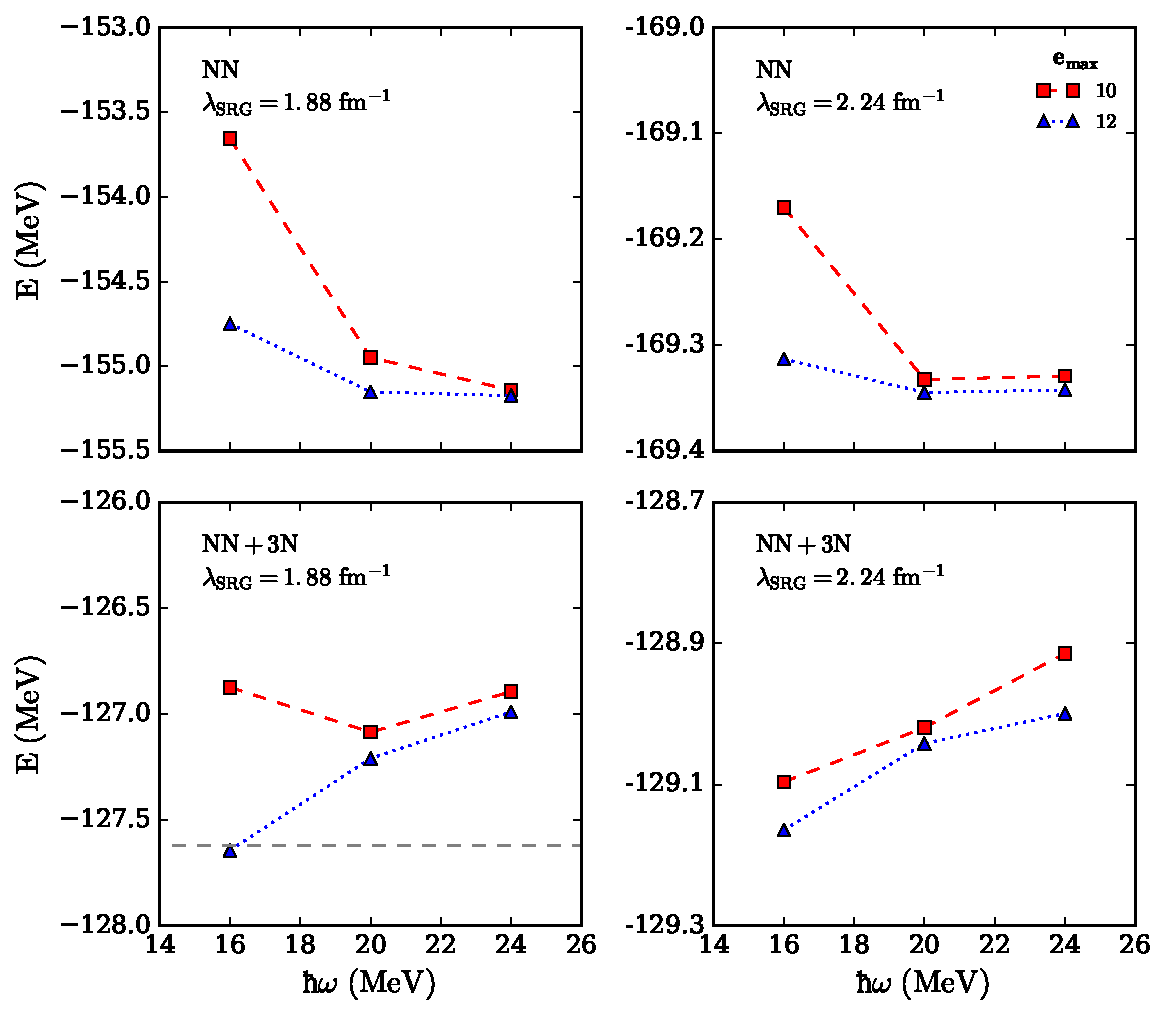
\includegraphics[width=\linewidth]{CC/ground_state_srg.pdf}
  \caption{Ground-state energies for ${}^{16}O$ for the EM N$^{3}$LO NN only interaction and with the added 3N interaction from Navr\'{a}til, both SRG softened with $\lambda_{\mathrm{SRG}}=1.88,2.24\ \mathrm{fm}^{-1}$.  The energies are plotted for $e_\mathrm{max}=10,12$.  The most obvious difference is between the NN and NN+3N calculations, showing the importance of including 3N forces.  The differences between the cutoff parameters are resolved within $\sim 1\%$ with the inclusion of 3N forces and can be rectified further by including additional correlations or full 3N forces.  The experimental binding energy is shown with the grey dashed line.}
  \label{fig:Ground_State_srg}
\end{figure}
Accounting for both the small dependence on the SRG cutoff parameter and the minor inaccuracies from the truncations made to the cluster operator and the Hamiltonian, the rest of this work will use the NN+3N(400)-induced interaction with an SRG cutoff parameter of $\lambda_{\mathrm{SRG}}=2.0\ \mathrm{fm}^{-1}$.

Next, any nuclear observables calculated with this framework should be independent of the fictitious confining potential.  This can be verified by showing the ground-state energies of various nuclei as a function of the underlying harmonic oscillator energy, $\hbar\omega$.  Convergence is reached by increasing the size of the model space until the resulting curve is flat.  Figure\ \ref{fig:Ground_State1} shows the convergence for the \textit{doubly-magic}, $N=Z$ nuclei, ${}^{4}$He, ${}^{16}$O, ${}^{20}$Ca, and ${}^{56}$Ni, where both protons and neutrons fill the same major shell closure.
\begin{figure}[h!]
  \centering
  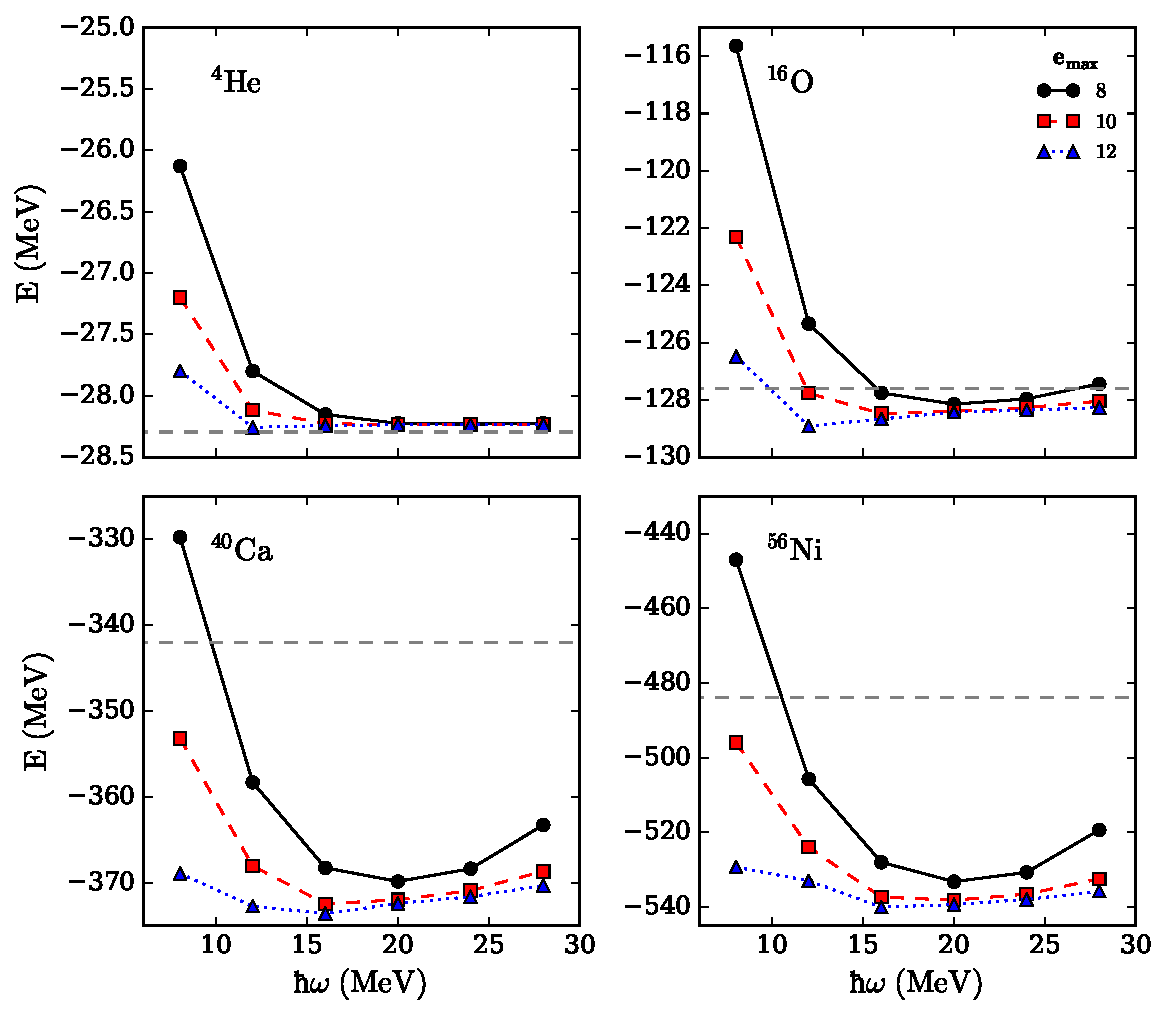
\includegraphics[width=\linewidth]{CC/ground_state1.pdf}
  \caption{Ground-state energies for doubly magic nuclei as a function of the harmonic oscillator energy $\hbar\omega$ with the NN+3N(400) interaction, SRG softened with $\lambda_{\mathrm{SRG}}=2\mathrm{fm}^{-1}$.  The energies are plotted for $e_\mathrm{max}=8,10,12$, showing the convergence as the model space increases.  The results are independent of the underlying oscillator frequency to $\sim 1\%$ for $e_\mathrm{max}=12$.  The grey dashed line is the experimental binding energy.  The overbinding of this interaction becomes apparant as the system size increases.}
  \label{fig:Ground_State1}
\end{figure}
All the results converge to a variance of $<1\%$ at $e_{\mathrm{max}}=12$ for intermediate values of $\hbar\omega$.  While a larger model space is always desirable, this level of variance justifies the use of $e_{\mathrm{max}}=12$ for post-CC calculations.  Additionally, these results show the limitations of the NN+3N(400) interaction, as overbinding increases with the system size, where the ground-state energies of ${}^{20}$Ca and ${}^{56}$Ni differ from their experimental binding energies by $\sim 8\%$ and $\sim 13\%$, respectively.

The ground-state results are also shown for singly-magic nuclei, where either the protons or neutrons fill a sub-shell closure.  This has the potential complication of a vanishing energy gap between the hole and particle states, like the picture in Fig.\ \ref{Harmonic_Oscillator}, which causes undefined behavior in the CC algorithm (see section \ref{section:solvingcc}).  However, the subshell orbitals repel each other when transformed during the Hartree-Fock algorithm \cite{LEVIT1999}, so these systems are valid in some cases.  The ground-state energies for ${}^{14}$C, ${}^{22}$O, and ${}^{34}$Si are plotted as a function of the underlying oscillator potential in Fig.\ \ref{fig:Ground_State2}.  The smaller energy gap involved in these systems results in stronger excitations missed by the CCSD approximation, causing further deviations from the experimental values.
\begin{figure}[h!]
  \centering
  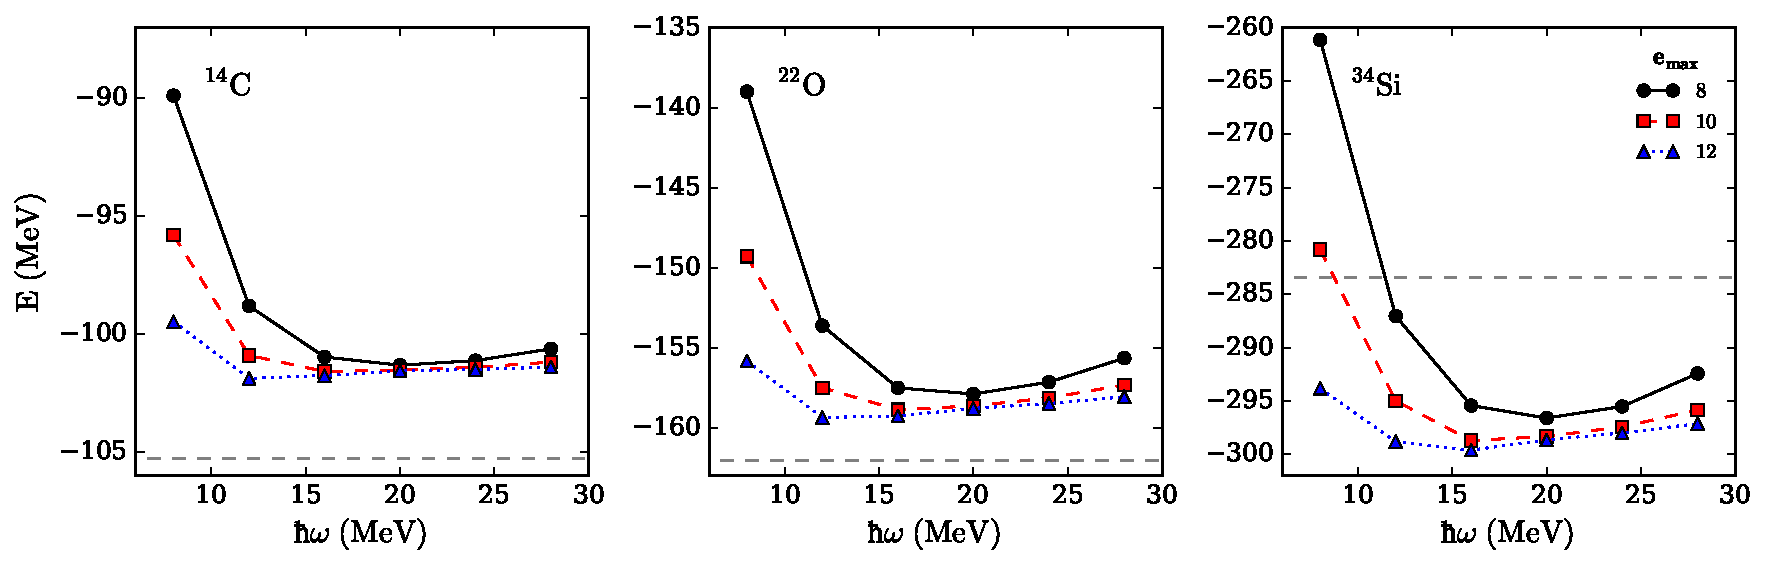
\includegraphics[width=\linewidth]{CC/ground_state2.pdf}
  \caption{Ground-state energies for singly magic nuclei as a function of the harmonic oscillator energy $\hbar\omega$ with the NN+3N(400) interaction, SRG softened with $\lambda_{\mathrm{SRG}}=2\mathrm{fm}^{-1}$.  The energies are plotted for different $e_\mathrm{max}$.  The results are independent of the underlying oscillator frequency to $\sim 1\%$ for $e_\mathrm{max}=12$.  The grey dashed line is the experimental binding energy.  These results underbind with respect to their doubly-magic counterparts in Fig.\ \ref{fig:Ground_State1}.}
  \label{fig:Ground_State2}
\end{figure}

\section{Ground-State Center-of-Mass Factorization} \label{section:CoM}
While an intrinsic Hamiltonian can be built by removing the center-of-mass (COM) kinetic energy, Eq.\ \eqref{eq:intrinsic_hamiltonian}, there is still an inconsistency between the translational invariance of the underlying harmonic oscillator basis and translationally-invariant nuclear many-body states \cite{LIPKIN1958,GLOECKNER1974313}.  This inconsistency can materialize in certain calculations in the form of spurious, non-physical states.

Of course, this problem can be avoided by using more complicated basis states that obey translational invariance, such as the use of Jacobi coordinates, but such methods are limited to few-body problems \cite{BISHOP19901341,NOGGA2002054003}.  Another possible solution is to use the harmonic oscillator basis in an untruncated space of Slater determinants up to a certain harmonic oscillator shell.  Known as the $N_{\mathrm{max}}$ space, this treatment can be successfully applied within no-core shell model calculations \cite{NAVRATIL2009083101}. However, the factorial scaling of this method restricts its use to light nuclei.  It can be shown that in the $N_{\mathrm{max}}$ space, the eigenstates of the intrisic Hamiltonian are also eigenstates of the COM Hamiltonian, and any state perfectly factorizes into a COM component and a translationally-invariant, intrinsic component,
\begin{equation} \label{eq:com_factorize}
  \corrket = \ket{\Corr_{\mathrm{in}}}\ket{\Corr_{\mathrm{cm}}}.
\end{equation}

This factorization results in a compound energy spectrum, where the intrinsic component of the spectrum is degenerate for each COM excitation.  Therefore, the intrinsic spectrum can be recovered by offsetting the COM Hamiltonian by the corresponding excitation energies, such that the COM energies vanish, $E_{\mathrm{cm}} = 0$.  However, with truncated methods like CCSD, this factorization is not guaranteed, and COM energies, no longer eigenenergies of the COM Hamiltonian, can take on values $E_{\mathrm{cm}} \neq 0$.  In this case, the intrinsic spectrum is contaminated with nonphysical, \textit{spurious} states.

Because the specific form is irrelevant \cite{VINCENT2973}, the shifted COM Hamiltonian can be assumed to take the form of a harmonic trap with a oscillator strength of $\hbar\widetilde{\omega}$, not necessarily equal to the oscillator strength of the underlying basis $\hbar\widetilde{\omega}$,
\begin{equation} \label{eq:com_hamiltonian}
  \Ham_{\mathrm{cm}}\left(\widetilde{\omega}\right) = \frac{\mathbf{P}_{\mathrm{cm}}}{2mA} + \frac{1}{2}mA\widetilde{\omega}^{2}\mathbf{R}_{\mathrm{cm}} - \frac{3}{2}\hbar\widetilde{\omega},
\end{equation}
offset by the ground-state energy, $\frac{3}{2}\hbar\widetilde{\omega}$.  In the $N_{\mathrm{max}}$ space, the factorization in Eq.\ \eqref{eq:com_factorize} occurs regardless of $\hbar\widetilde{\omega}$, while in truncated methods like CCSD, the COM oscillator strength is a free parameter which can be used to probe the level of COM contamination.  If a frequency exists such that $E_{\mathrm{cm}}\left(\widetilde{\omega}\right) \approx 0$, then the wave function is approximately factorized, and the COM wave function is in its ground state \cite{HAGEN2009062503,JANSEN2013}.

The COM energy, $E_{\mathrm{cm}}$, can be calculated by using a version of the Hellmann-Feynman theorem by adding the COM Hamiltonian as a perturbation and computing the difference quotient \cite{DIERCKSEN198129,ERNZERHOF199359},
\begin{equation} \label{eq:com_energy}
  E_{\mathrm{cm}}\left(\widetilde{\omega}\right) \equiv \element{\Corr}{\Ham_{\mathrm{cm}}}{\Corr} \approx \frac{1}{2\delta}\left(\element{\Corr}{\Ham + \delta\Ham_{\mathrm{cm}}\left(\widetilde{\omega}\right)}{\Corr} - \element{\Corr}{\Ham - \delta\Ham_{\mathrm{cm}}\left(\widetilde{\omega}\right)}{\Corr}\right).
\end{equation}
Because the operator $\mathbf{R}_{\mathrm{cm}}$ depends only on the underlying single-particle basis regardless of the COM oscillator frequency, it can be rewritten in terms of $\Ham_{\mathrm{cm}}$ to find the relationship between $\omega$ and $\widetilde{\omega}$,
\begin{equation}
  \frac{1}{\widetilde{\omega}^{2}}\left(\Ham_{\mathrm{cm}}\left(\widetilde{\omega}\right) - \Top_{\mathrm{cm}} + \frac{3}{2}\hbar\widetilde{\omega}\right) = \frac{1}{\omega^{2}}\left(\Ham_{\mathrm{cm}}\left(\omega\right) - \Top_{\mathrm{cm}} + \frac{3}{2}\hbar\omega\right).
\end{equation}
Using the known value $\element{\Corr}{\Top_{\mathrm{cm}}}{\Corr} = \frac{3}{4}\hbar\widetilde{\omega}$ and the requirement that $E_{\mathrm{cm}}\left(\widetilde{\omega}\right)=0$ gives the following relation that relates the COM oscillator frequency to the underlying basis frequency,
\begin{equation} \label{eq:com_hw}
  \hbar\widetilde{\omega} = \hbar\omega + \frac{2}{3}E_{\mathrm{cm}}\left(\omega\right) \pm \sqrt{\left(\frac{2}{3}E_{\mathrm{cm}}\left(\omega\right)\right)^{2} + \frac{4}{3}\hbar\omega E_{\mathrm{cm}}\left(\omega\right)}.
\end{equation}

The ground-state COM energies are plotted for ${}^{16}$O and ${}^{40}$Ca using the COM Hamiltonian with two different oscillator strengths in Fig.\ \ref{fig:CoM_Ground_State}: that of the underlying basis, $\hbar\omega$, and one of the two solutions to Eq.\ \eqref{eq:com_hw}, $\hbar\widetilde{\omega}_{\pm}$.  Of the two $\hbar\widetilde{\omega}_{\pm}$, which are shown as the solutions to Eq.\ \eqref{eq:com_hw} in the inset, one typically results in a large COM energy while the other vanishes, which is plotted.  Because the COM energies approximately vanish regardless of the underlying basis frequency, the COM wave function is in its ground state and approximately factorized from the intrinsic nuclear wave function.
\begin{figure}[h]
  \centering
  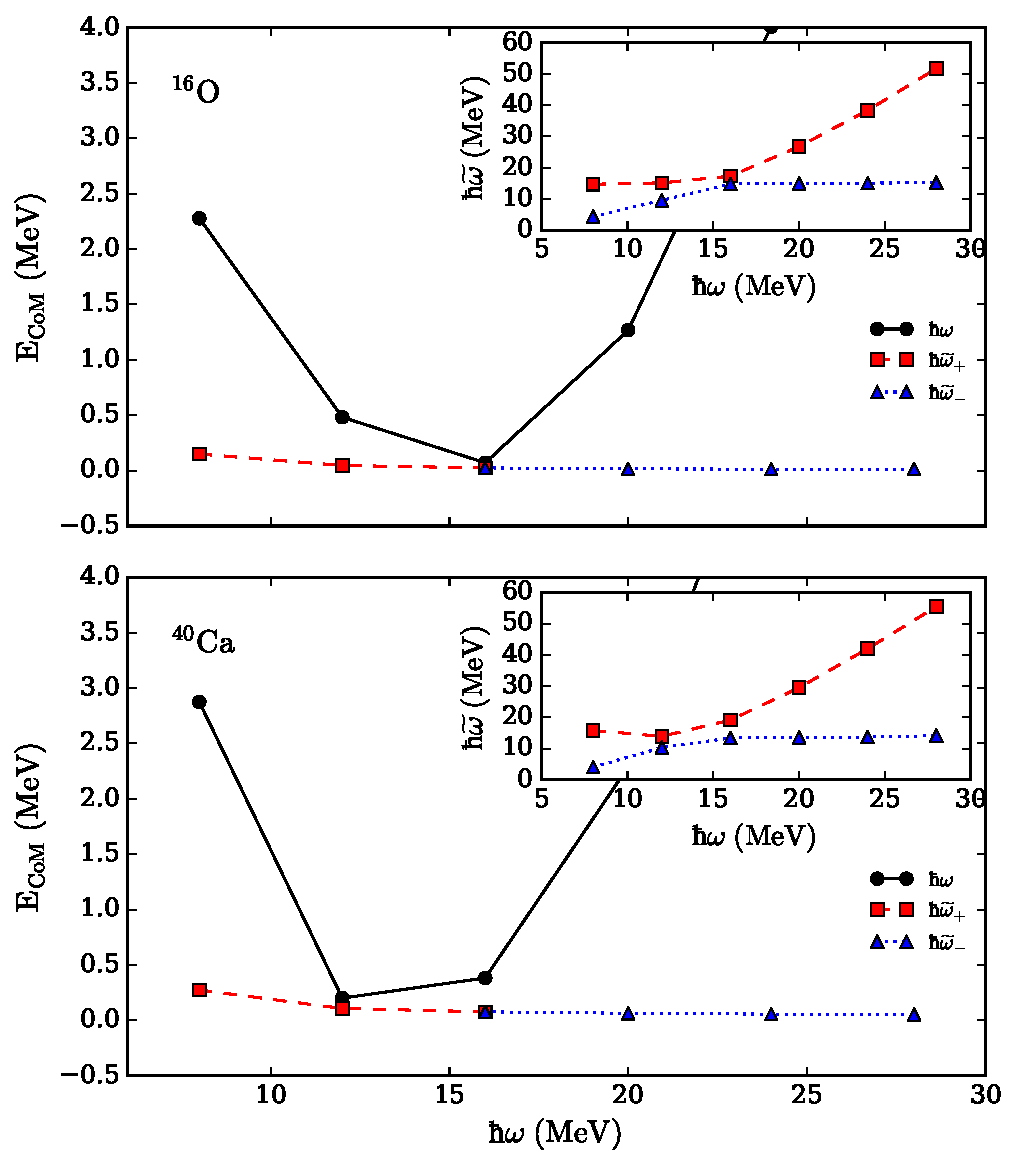
\includegraphics[width=\textwidth]{CC/CoM1.pdf}
  \caption{Ground-state COM energies, Eq.\ \eqref{eq:com_hamiltonian}, for ${}^{16}$O and ${}^{40}$Ca at varies harmonic oscillator frequencies with the NN+3N(400)-induced with $\lambda_{\mathrm{SRG}}=2.0\ \mathrm{fm}^{-1}$ at $e_{\mathrm{max}}=12$.  Using the proper COM oscillator frequencies shows the approximate factorization of Eq.\ \eqref{eq:com_factorize}.}
  \label{fig:CoM_Ground_State}
\end{figure}

Unfortunately, when intrinsic states are coupled to COM excited-states, they can contaminate the spectrum of intrinsic states that are coupled to the COM ground-state.  These spurious states can be essentially removed from the ground-state spectrum with the Lawson-Gloeckner method \cite{GLOECKNER1974313}.  When the proper COM oscillator strength is chosen such that the COM ground-state energy vanishes, the COM Hamiltonian can be added to the intrinsic Hamiltonian at an arbitrarily large scale, $\beta$, without changing the ground-state spectrum,
\begin{equation} \label{eq:lawson-term}
  \Ham_{\mathrm{in}} \rightarrow \Ham_{\mathrm{in}} + \beta\Ham_{\mathrm{cm}}.
\end{equation}
When $\beta$ is arbitrarily large, eigenenergies of intrinsic states coupled to COM excited states will increase by the COM energy quanta, $\beta\hbar\widetilde{\omega}$, such that they are removed from the range of low-lying states of interest.  The method will be used to remove spurious states from the spectra of open-shell states in section \ref{chapter:eom}.
  
\end{document}
